\documentclass[11pt]{article}
\usepackage{mystyle}

\title{Programming Project 1: Vibrational Frequencies and Normal Modes}
\date{}

\begin{document}
\maketitle

\section*{Description}
The aim of this programming project is compute harmonic vibrational frequencies
using second derivatives of the potential energy surface. See
section~\ref{background} for details on the theory.

In essence, the task of this project is boils down to two steps:
\begin{enumerate}
    \item formation of the mass-weighted Hessian matrix, which has elements
\begin{align}
(\tl{\bo{H}}_0)_{AB}
    = \left(\dfrac{\pt^2E_e}{\pt\tl{X}_A \pt\tl{X}_B}\right)_0
    = \dfrac{1}{\sqrt{M_A}} \left(\dfrac{\pt^2E_e}{\pt X_A\pt X_B}\right)_0 \dfrac{1}{\sqrt{M_B}}
\end{align}
where $M_{3A-2} = M_{3A-1} = M_{3A}$ and $X_{3A-2}, X_{3A-1}, X_{3A}$ are the
mass and $X,Y,Z$ coordinates of the $A$\eth\ nucleus, and
$\tl{X}_A = \sqrt{M_A} X_A$ represents a mass-weighted coordinate.
    \item diagonalization of the mass-weighted Hessian matrix
\begin{align}
\tl{\bo{H}}_0
    = \bo{L} \bm\La \bo{L}^T \sp \bm{\La}
    = \ma{\la_1&   0   &  \ld  &    0     \\
            0  & \la_2 &  \ld  &    0     \\
           \vd &  \vd  &  \dd  &   \vd    \\
            0  &   0   &  \ld  & \la_{3N} }
\end{align}
where column vectors of the $\bo{L}$ matrix are orthonormal eigenvectors
$\bm{l}_1, \ld, \bm{l}_{3N}$ of the mass-weighted Hessian matrix, and
$\la_1, \ld, \la_{3N}$ are the corresponding eigenvalues.
\end{enumerate}
In matrix notation, the mass-weighting can be written as
\begin{align}
    \tl{\bo{H}}_0
=   \bo{M}^{-\frac{1}{2}} \bo{H}_0 \bo{M}^{-\frac{1}{2}}
\sp \bo{M}
\equiv
    \ma{ M_1 &  0  & \ld &   0    \\
          0  & M_2 & \ld &   0    \\
         \vd & \vd & \dd &  \vd   \\
          0  & 0   & \ld & M_{3N} }
\end{align}
where $\bo{H}_0$ is the Hessian matrix in ordinary Cartesian coordinates. For
eigenvalues $\la_A > 0$, $\la_A$ corresponds to the square of the frequency of
molecular vibration $\la_A = \w_A^2$ along the direction of motion represented
by the corresponding eigenvector, which is $\bo{M}^{-\frac{1}{2}} \bm{l}_A$.
This direction of motion corresponds to a {\it vibrational normal coordinate},
typically represented by $Q_A$, and motion along this coordinate corresponds to
a displacement of
\begin{align}
    \D\bo{X}(Q_A) = Q_A\bo{M}^{-\frac{1}{2}}\bm{l}_A
\end{align}
relative to the reference configuration $\bo{X}_0$. In addition to the
vibrational modes, there will be three {\it translational normal coordinates}
for which $\la_A=0$ and three {\it rotational normal coordinates} (two for
linear systems) for which $\la_A=0$ holds at an equilibrium geometry.

In order to complete this project you will need a hessian, molecule, code you
wrote to extract information from an xyz file, and a file called \ttf{masses.py}
containing masses for the most stable isotope of every element will also be
provided. The files are available in the aptly named folder
\texttt{extra-files/}.

\newpage
\section{Procedure}

Make a file called \texttt{proj1.py} with the following code, which will tell
Python where the necessary files are (obviously change the name to yours).

\linp[firstline=1, lastline=5]{../jevandezande/proj1.py}

\subsection{Read in the molecule}
Import your script, read in the file \texttt{molecule.xyz} and convert to
Angstroms.

\subsection{Read in the Hessian matrix}
Read in each of the elements of the hessian matrix (\texttt{hessian.dat}) and
save as a numpy matrix.

\subsection{Generate $\bo{M}^{-\frac{1}{2}}$}
Use the molecule that you read in to get the atoms of the molecule. You can
then use the function get\_mass from the file \texttt{masses.py} to find the
mass of each of your atoms. Use these masses to generate $\bo{M}^{-\frac{1}{2}}$.
\begin{align}
    \bo{m} = \left[\fr{1}{\sqrt{M_1}}, \fr{1}{\sqrt{M_2}}, \fr{1}{\sqrt{M_3}},
\ld, \fr{1}{\sqrt{M_{3N}}} \right]
    \text{\small\ where $M_{3A-2} = M_{3A-1} = M_{3A}$ is the mass of the $A$\eth\ atom}
\end{align}
using the \ttf{get\_mass()} function in \ttf{masses.py}, which can be called as follows.
\begin{lstlisting}[language=python]
>>> import masses
>>> masses.get_mass("C")
12
>>> masses.get_mass("H")
1.00782503207
>>> masses.get_mass("O")
15.99491461956
>>> masses.get_mass("N")
14.00307400478
>>> masses.get_mass("P")
30.973761629
\end{lstlisting}
The square root of a number can be determined either by using the exponential
operator in Python \ttf{a**b}~$=a^b$ or by using the square root function
\footnote{\url{http://docs.scipy.org/doc/numpy/reference/generated/numpy.sqrt.html}}
provided by the NumPy package.

\subsection{Form $\bo{H}_0$ and $\bo{M}^{-\frac{1}{2}}$ as NumPy matrices}
This can be achieved using the Numpy functions \ttf{numpy.matrix()}
\footnote{\url{http://docs.scipy.org/doc/numpy/reference/generated/numpy.matrix.html}}
and \ttf{numpy.diag()}.
\footnote{\url{http://docs.scipy.org/doc/numpy/reference/generated/numpy.diag.html}}

\subsection{Form the mass-weighted Hessian $\tl{\bo{H}}_0 = \bo{M}^{-\frac{1}{2}}\bo{H}_0\bo{M}^{-\frac{1}{2}}$}

For NumPy matrices \ttf{A} and \ttf{B}, \ttf{A*B} returns the matrix product.

\subsection{Determine the eigenvalues and eigenvectors of $\tl{\bo{H}}_0$}

This can be achieved using the \ttf{eigh()} function
\footnote{\url{http://docs.scipy.org/doc/numpy/reference/generated/numpy.linalg.eigh.html\#numpy.linalg.eigh}}
in the \ttf{numpy.linalg} module.

\subsection{Determine the vibrational frequencies}

The eigenvalues that we extracted correspond to frequencies. However,
wavenumbers are not a true unit of frequency, which physically corresponds to
inverse time rather than inverse length. The ``conversion factor'' between
frequencies in wavenumbers (denoted $\tl\nu$) and true frequencies $\nu$ is the
speed of light in a vacuum $c$.
\begin{align*}
    \tl\nu = \fr{\nu}{c}
\end{align*}
Be sure that you are aware of the difference between angular frequency
(radians/time) and true temporal frequency (cycles/time) before attempting
this.

\subsection{Generate an \ttf{.xyz} file containing the normal modes}
\label{generate-xyz-modes}
Note that the Cartesian displacements represented by normal modes correspond to
$\bo{M}^{-\frac{1}{2}}\bm{l}_A$ rather than the eigenvectors $\bm{l}_A$
themselves. All distance units for this file must be in \AA ngstr\"oms, so you
will have to apply a unit conversion to both the reference configuration and
the mode displacements before printing. The format of this extended \ttf{.xyz}
file used for mode visualization is described below.

\subsection{Visualize in Jmol}
Obviously, you should visualize the modes after completing step
\ref{generate-xyz-modes}. If you have Jmol installed, the file generated in
that step (call it \ttf{modes.xyz}) can be opened at the command line with the
command \ttf{jmol modes.xyz}. In Jmol, select \ttf{Vibrate...} under
\ttf{Tools} and click on \ttf{Start vibration}. The comment line corresponding
to each mode will appear in the lower left corner, and you can cycle through
the various modes with the left and right arrow icons.

You should also check your vibrational modes by running a frequency computation
in Psi4 with the same method and level of theory. The simplest way to do this
is to copy the input file for your reference geometry computation in the
previous project and replace \ttf{energy('scf')} with \ttf{frequencies('scf')}.
You may be surprised at first to find that your rotational normal modes are
significantly different from zero. The reason for this is that the geometry you
were given is not an equilibrium structure for H$_2$O at the RHF/cc-pVDZ level,
and the eigenvalues corresponding to rotational modes are, in general, nonzero
away from equilibrium. The motivation for starting with a non-equilibrium
geometry is that the lifting the degeneracy between rotational and
translational motion reduces the numerical error in the diagonalization
procedure for determining the corresponding eigenvectors. As a final step to
this project, you should determine the equilibrium geometry for water at the
RHF/cc-pVDZ level and compute new frequencies by first running your scripts for
determining the Hessian numerically and then running your frequency
computation. You should notice two things:
\begin{enumerate}
    \item you should now have six frequencies near zero (within $50$~cm$^{-1}$
real or imaginary)
    \item your rotational and translational modes will now be barely
recognizable when you visualize them in Jmol
\end{enumerate}
After this is done, congratulate yourself and take a break.


\newpage
\section{Extra Files and File Formats}
\subsection{\ttf{masses.py}}
This file provides an easy way to retrieve the mass (in atomic mass units) of
the most stable isotope of an element by atomic symbol. You should look at this
file and be sure you understand what it does. It contains a dictionary
\footnote{\url{https://docs.python.org/2/tutorial/datastructures.html\#dictionaries}}
to convert from atomic symbol to atomic number as well as a list of isotopic
masses (corresponding to the most stable isotope) indexed by atomic number. The
\ttf{get\_mass()} function assumes a string argument, converts the string to
uppercase, grabs the corresponding atomic number, and then returns the
corresponding mass in the list.


\subsection{\ttf{.xyz} files for visualizing vibrational modes}
The file format for visualizing a single normal mode in Jmol is
\begin{addmargin}{5cm}{}
\begin{lstlisting}[language=c++]
N
COMMENT LINE 1
A1 x1 y1 z1   dx1 dy1 dz1
A2 x2 y2 z2   dx2 dy2 dz2
...                        
AN xN yN zN   dxN dyN dzN
\end{lstlisting}
\end{addmargin}
which amounts to a standard \ttf{.xyz} geometry file (described in the previous
handout) with the Cartesian displacement vector for each atom printed next to
its Cartesian coordinates. For visualizing multiple motions, this format is
simply repeated with an intervening empty line.
\begin{addmargin}{5cm}{}
\begin{lstlisting}[language=c++]
N
COMMENT LINE 1
A1 x1 y1 z1   dx11 dy11 dz11
A2 x2 y2 z2   dx12 dy12 dz12
...                        
AN xN yN zN   dx1N dy1N dz1N
                           
N                          
COMMENT LINE 2             
A1 x1 y1 z1   dx21 dy21 dz21
A2 x2 y2 z2   dx22 dy22 dz22
...                        
AN xN yN zN   dx2N dy2N dz2N
                           
...                        
                           
N                          
COMMENT LINE N             
A1 x1 y1 z1   dxN1 dyN1 dzN1
A2 x2 y2 z2   dxN2 dyN2 dzN2
...                        
AN xN yN zN   dxNN dyNN dzNN
\end{lstlisting}
\end{addmargin}
Note that, in order to use this file for visualization, the length units must
be \AA ngstr\"oms.

\newpage
\section{Background}\label{background}

\subsection{The Born-Oppenheimer Approximation}
Under the Born-Oppenheimer approximation the stationary-states
\footnote{\url{http://en.wikipedia.org/wiki/Stationary_state}} of nuclear
motion $\Y_\Nu$ arise as solutions of the nuclear motion equation.
\begin{align}
\label{pes}
    \op{H}_\Nu
    \Y_\Nu(\bo{X})
=
    E
    \Y_\Nu(\bo{X})
\sp
    \op{H}_\Nu
\equiv
    \op{T}_\Nu+E_e(\bo{X})
\end{align}
The potential energy term $E_e(\bo{X})$ in the nuclear motion Hamiltonian is
defined through the clamped-nuclei Schr\"odinger equation.
\begin{align}
\label{clamped-se}
    \op{H}_e(\bo{X})
    \Y_e(\bo{r}_1,\ld,\bo{r}_n;\bo{X})
=
    E_e(\bo{X})
    \Y_e(\bo{r}_1,\ld,\bo{r}_n;\bo{X})
\end{align}
Equation (\ref{clamped-se}) can be solved approximately at any point
$\bo{X}=(\bo{R}_1,\ld,\bo{R}_N)$ using your favorite electronic structure
software package (\textsc{Psi4}, CFOUR, Molpro, Gaussian, etc.) and electronic
structure method (MP2, CCSD, CISD, etc.).


\subsection{Normal Coordinates and the Vibrational Schr\"odinger Equation}

One of the major barriers to solving the nuclear motion equation (\ref{pes}) is
the difficulty of determining the potential energy surface $E_e(\bo{X})$ at a
sufficiently large number of points. Since the nuclei generally remain
relatively localized about an equilibrium configuration $\bo{X}_0$, a good
first approach is to approximate the potential surface by a Taylor expansion.
\begin{align*}
    E_e(\bo{X})
\approx
    E_e(\bo{X}_0)
+\sum_A^{3N}
    \pr{\pd{}{E_e}{X_A}}_0
    \D X_A
+\fr{1}{2}\sum_{AB}^{3N}
    \pr{\fr{\pt^2E_e}{\pt X_A\pt X_B}}_0
    \D X_A
    \D X_B
    \sp \D\bo{X}=\bo{X}-\bo{X}_0
\end{align*}
Equilibrium structures occur at minima on the potential energy surface, so that
the second term is zero and only the quadratic term remains.
\begin{align}
    E_e(\bo{X})
\approx
    E_e(\bo{X}_0)
+\fr{1}{2}\sum_{AB}^{3N}
    \pr{\fr{\pt^2E_e}{\pt X_A\pt X_B}}_0
    \D X_A
    \D X_B
\end{align}
For convenience, we use mass-weighted coordinates $\tl{X}_A \equiv \sqrt{M_A}\D
X_A$ in order to remove the explicit dependence of the kinetic energy operator
on nuclear masses. \footnote{Explicitly, we can write
$\fr{\op{\bo{P}}_A^2}{2M_A} = -\fr{1}{2M_A}
\pd{2}{}{X_A}=-\fr{1}{2}\pd{2}{}{(\sqrt{M_A}\D
X_A)}=-\fr{1}{2}\pd{2}{}{\tl{X}_A}$. ($\hbar=1$ since we are working in atomic
units)}
\begin{align}
    \op{T}_\Nu
=
    -\fr{1}{2}\sum_A^{3N} \pd{2}{}{\tl{X}_A}
\end{align}
The nuclear motion equation (\ref{pes}) then becomes
\begin{align}
\label{pes-intermediate}
\pr{
-\fr{1}{2}\sum_A^{3N}
    \pd{2}{}{\tl{X}_A}
+\fr{1}{2}\sum_{AB}^{3N}
    \pr{\fr{\pt^2E_e}{\pt \tl{X}_A\pt \tl{X}_B}}_0
    \tl{X}_A
    \tl{X}_B
}
    \Y_\Nu(\tl{\bo{X}})
=
    E_\Nu
    \Y_\Nu(\tl{\bo{X}})
\sp
    E_\Nu
\equiv
    E - E_e(\bo{X}_0)
\end{align}
which brings us to the crucial step that motivates this project.

\paragraph{the crucial step that motivates this project:} Note that, if the
mass-weighted Hessian matrix
\begin{align}
    (\tl{\bo{H}}_0)_{AB}
=
    \pr{\fr{\pt^2 E_e}{\pt\tl{X}_A\pt\tl{X}_B}}_0
\end{align}
were diagonal, we would have a sum of harmonic oscillator Hamiltonians
\footnote{The Hamiltonian of a single harmonic oscillator is
$\op{H}=\fr{\op{p}^2}{2m}+\fr{m\w^2\op{x}^2}{2}$, or
$\op{H}=-\fr{1}{2}\pd{2}{}{q}+\fr{\w^2}{2}q^2$ in mass-weighted coordinates
with atomic units.  The frequency of oscillation is $\w$.} in equation
(\ref{pes-intermediate}). This dream of a simple Hamiltonian can be realized by
choosing a new set of coordinates in terms of which the Hessian is diagonal.
Since the mass-weighted Hessian $\tl{\bo{H}}_0$ is real and symmetric, it can
be diagonalized by a real orthogonal matrix $\bo{L}$
\footnote{\url{http://en.wikipedia.org/wiki/Symmetric_matrix\#Decomposition}}
\begin{align}
    \tl{\bo{H}}_0
=
    \bo{L}\bm{\La}\bo{L}^T
\sp
    \bm{\La}
=
    \ma{ \la_1 &   0   &  \ld  &   0      \\
           0   & \la_2 &  \ld  &   0      \\
          \vd  &  \vd  &  \dd  &  \vd     \\
           0   &   0   &  \ld  & \la_{3N} }
\sp
    \bo{L}\bo{L}^T=\bo{L}^T\bo{L}=\bo{1}
\end{align}
where the columns of $\bo{L}$ are eigenvectors $\bm{l}_1,\ld,\bm{l}_{3N}$ of
$\tl{\bo{H}}_0$. The mass-weighted Hessian can be put into this form by
expressing our coordinates in the basis of its eigenvectors. These new
coordinates are called {\it normal coordinates}, and the coordinate vector is
traditionally referred to as $\bo{Q}$. The relationship between normal
coordinates and mass-weighted Cartesian displacement coordinates is
$\bo{Q}=\bo{L}^T\tl{\bo{X}}$, so that the relationship to Cartesian
displacements is
\begin{align}
\label{q-to-dx}
    \bo{Q}
=
    \bo{L}^T
    \bo{M}^{\frac{1}{2}}
    \D\bo{X}
\sp
    \bo{M}^{\frac{1}{2}}
\equiv
    \ma{ \sqrt{M_1} &     0      &   \ld  &     0         \\
             0      & \sqrt{M_2} &   \ld  &     0         \\
            \vd     &    \vd     &   \dd  &    \vd        \\
             0      &     0      &   \ld  & \sqrt{M_{3N}} }
\end{align}
Cartesian displacements therefore depend on the normal coordinates by the
following relationship.
\begin{align*}
    \D\bo{X}
=
    (\bo{L}^T\bo{M}^{\frac{1}{2}})^{-1}\bo{Q}
=
    \bo{M}^{-\frac{1}{2}}\bo{L}\bo{Q}
\end{align*}
This shows that a motion along the various coordinates $Q_1,\ld,Q_{3N}$
corresponds to a Cartesian displacement by
\begin{align}
    \D\bo{X}(Q_1,\ld,Q_{3N})
=
    Q_1\pr{\bo{M}^{-\frac{1}{2}}\bm{l}_1}
+
    Q_2\pr{\bo{M}^{-\frac{1}{2}}\bm{l}_2}
+
    \ld
+
    Q_{3N}\pr{\bo{M}^{-\frac{1}{2}}\bm{l}_{3N}}
\end{align}
where the $\bm{l}_A$ represent column vectors of $\bo{L}$, i.e.
$\bo{L}=\ma{\bm{l}_1&\ld&\bm{l}_{3N}}$. We see that each $Q_A$ corresponds to a
collective displacement $\D\bo{X}=\bo{M}^{-\frac{1}{2}}\bm{l}_A$ of several
nuclei. The noral coordinates for water are included in an appendix to this
handout, and a more detailed interpretation of what these motions represent
will be given in the next section. Note that the Hessian matrix $\bo{H}$
changes continuously across the potential energy surface, so that each point on
the surface is associated with its own set of normal coordinates. Although the
normal coordinates at every point span the full space $\mathbb{R}^{3N}$ of
nuclear configurations, \footnote{i.e., any set of nuclear positions can be
specified by a set of values for $Q_1,\ld,Q_{3N}$} the normal coordinates at a
particular point on the potential surface are generally only physically
appropriate for describing nuclear motion within a small region about that
configuration.

Expressing equation (\ref{pes-intermediate}) in terms of these newfangled
coordinates, we are left with 
\begin{align}
\label{vib-se}
\pr{
-\fr{1}{2}\sum_A^{3N}
    \pd{2}{}{Q_A}
+\fr{1}{2}\sum_A^{3N}
    \la_A Q_A^2
}
    \Y_\Nu(\bo{Q})
=
    E_\Nu
    \Y_\Nu(\bo{Q})
\end{align}
(details of the coordinate transformation are shown in an appendix). The
Hamiltonian in (\ref{vib-se}) has the marvelously simple form we were hoping
for:
\begin{align}
\label{harm-hamiltonian}
    \op{H}_\Nu
\approx
    \sum_{A=1}^{3N}
    \op{\mf{h}}_A
\sp
    \op{\mf{h}}_A
\equiv
-\fr{1}{2}
    \pd{2}{}{Q_A}
+\fr{1}{2}
    \la_A Q_A^2
\end{align}
The only approximation for $\op{H}_\Nu$ here is the truncation of the potential
energy surface Taylor expansion at second order. As long as $\la_A$ is a
positive real number, $\op{\mf{h}}_A$ is a harmonic oscillator Hamiltonian and
we can make the identification $\la_A=\w_A^2$ where $\w_A$ is the oscillator
frequency in a.u. It will turn out that, at an equilibrium geometry,
$\tl{\bo{H}}_0$ has several zero eigenvalues -- one for each translational and
rotational degree of freedom for the entire nuclear framework with respect to
its center of mass. For these motions, $\op{\mf{h}}_A$ actually takes the form
of a free-particle Hamiltonian
\footnote{\url{http://en.wikipedia.org/wiki/Free_particle\#Non-Relativistic_Quantum_Free_Particle}}
\begin{align}
    \op{\mf{h}}_A
    = -\fr{1}{2} \pd{2}{}{Q_A}
\end{align}
although this form is somewhat misleading for rotational motion. In order to
get a clearer picture of what a normal coordinate physically represents, it
helps to shift to a classical picture for a moment.

\subsubsection{Classical Interpretation of Normal Coordinate Motions}
Let $\D\bo{X}$ represent a displacement from the equilibrium geometry
$\bo{X}_0$ to some new geometry $\bo{X}$:
\begin{align}
    \D\bo{X}
\equiv
    \bo{X}-\bo{X}_0
\end{align}
Then note that $\bo{H}_0\cdot\D\bo{X}$ represents the change in the potential
energy surface gradient between those two points
\begin{align*}
    \bo{H}_0\cdot\D\bo{X}
    = \nabla E_e - (\nabla E_e)_0
\end{align*}
which can be seen by expanding the gradient at $\bo{X}$ relative to the
gradient at $\bo{X}_0$:
\begin{align}
    \pd{}{E_e}{X_A}
    \approx \pr{\pd{}{E_e}{X_A}}_0
            +\sum_B
            \pr{\pd{}{}{X_B}\pd{}{E_e}{X_A}}_0
            \D X_B
\end{align}
Since $\bo{X}_0$ is an equilibrium geometry, the gradient $(\nabla E_e)_0$
vanishes at that point, and we have simply
\begin{align*}
    \bo{H}_0\cdot\D\bo{X}
    = \nabla E_e
\end{align*}
Mass-weighting our coordinate axes leaves the same form of expression.
\begin{align*}
    \tl{\bo{H}}_0\cdot\D\tl{\bo{X}}
    = \tl\nabla E_e
\end{align*}
Now, consider what it means for our displacement to be an eigenvector of
$\tl{\bo{H}}$.
\begin{align}
    \tl{\bo{H}}_0\cdot\D\tl{\bo{X}}
    = \la \D\tl{\bo{X}}
\end{align}
This means that $\D\tl{\bo{X}}$ is proportional to the potential energy surface
gradient at the displaced geometry
\begin{align*}
    \la \D\tl{\bo{X}}
    = \tl{\nabla}E_e
\end{align*}
Explicitly, this can be written as
\begin{align*}
    \la \sqrt{M_A} (X_A-(\bo{X}_0)_A)
    = \pd{}{E_e}{\sqrt{M_A}X_A}
\end{align*}
If we multiply both sides of the equation by $\sqrt{M_A}$, we find that
\begin{align}
    \la M_A (X_A-(\bo{X}_0)_A)
    = \pd{}{E_e}{X_A}
\end{align}
From a classical perspective, the gradient of the potential energy {\small
$\pd{}{E_e}{X_A}$} is simply a Cartesian component of (minus) the force
\footnote{\url{http://en.wikipedia.org/wiki/Classical_mechanics\#Work_and_energy}}
acting on one of the nuclei. Using Newton's second law, this gives
\begin{align*}
    \la M_A (X_A-(\bo{X}_0)_A)
    = -M_A (\bo{\ddot{X}})_A
\end{align*}
where $\bo{\ddot{X}}\equiv \fr{d^2\bo{X}}{dt^2}$.
Dividing both sides by $M_A$, we see that the displacement corresponds to a
motion parallel to the acceleration
\begin{align}
\label{norm-coords}
    -\la
    (\bo{X}-\bo{X}_0)
=   \bo{\ddot{X}}
\end{align}
Compare this to Hooke's law for a 1D oscillator, which is
$m\ddot{x}=-m\w^2(x-x_0)$. We see, then, that normal coordinates with positive
eigenvalues $\la>0$ correspond to directions of motion along which the
potential is ``spring-like'', inducing a force that accelerates the nuclei back
to their equilibrium position along the direction of displacement. It is useful
to consider the cases $\la=0$ and $\la<0$ as well. When $\la=0$, as for
translational and rotational modes at equilibrium, there is no force to
constrain the motion along these coordinates. When $\la$ is negative, as will
be true of one or more modes at non-equilibrium points, equation
(\ref{norm-coords}) shows that displacement induces an acceleration of the
nuclei {\it away} from the reference geometry.

\subsubsection{Solutions for Nuclear Motion in a Quadratic Well}
Here I will simply report the quantum mechanical solution to the translational
and vibrational components of equation (\ref{vib-se}).
\begin{align*}
\pr{\sum_{A=1}^{3N}
    \op{\mf{h}}_A }
    \Y_\Nu(\bo{Q})
=
    E_\Nu
    \Y_\Nu(\bo{Q})
\sp
    \op{\mf{h}}_A
=
-\fr{1}{2}
    \pd{2}{}{Q_A}
+\fr{1}{2}
    \la_A Q_A^2
\end{align*}
Since the Hamiltonian separates into a sum of independent Hamiltonians each
involving only one coordinate, the form of the wavefunction is
\begin{align}
    \Y_\Nu(Q_1,\ld,Q_{3N})
=
    \y_1(Q_1)
    \y_2(Q_2)
    \cdots
    \y_{3N}(Q_{3N})
\end{align}
where each one-coordinate wavefunction $\y_A(Q_A)$ is an eigenfunction (or,
rather, {\it one of the} eigenfunctions) of the corresponding operator,
$\op{\mf{h}}_A$.
\begin{align}
    \op{\mf{h}}_A
    \y_A(Q_A)
=
    \e
    \y_A(Q_A)
\end{align}
We will only need solutions to the 1D free-particle and 1D harmonic oscillator
Schr\"odinger equations for the present discussion, which can be found in any
introductory quantum mechanics text worth reading.\footnote{e.g. R.\ Shankar
{\it Principles of Quantum Mechanics}, which contains detailed discussions of
both the free particle and harmonic oscillator. An electronic copy can be found
\href{http://home.basu.ac.ir/\~psu/Books/\%5BRamamurti_Shankar\%5D_Principles_of_Quantum_Mechanic\%28BookFi.org\%29.pdf}{here}.}

For the three normal coordinates that correspond to translations of the
molecule as a whole, the potential term in $\op{\mf{h}}$ vanishes (since
$\la=0$) and we only need to solve a free-particle-like problem.
\begin{align}
-\fr{1}{2}
    \pd{2}{\y(Q_A)}{Q_A}
=
    \e
    \y(Q_A)
\end{align}
Solutions to this differential equation are given by
\begin{align}
    \y_{P_A}(Q_A)
=
    e^{iP_A(Q_A-\theta_A)}
\end{align}
where $\theta_A$ is some undetermined phase shift. The distribution of
eigenvalues is continuous in this case, $\e_{P_A}=\fr{P_A^2}{2}$, where $P_A$
corresponds to a component of the linear momentum of the molecule as a whole.

Although $\la=0$ also holds for rotational modes at equilibrium, normal
coordinates are only appropriate for parametrizing infinitesimal rotations and
quickly break down for larger rotational motions (see the images in section
\ref{rot}). Furthermore, unlike translations, these modes are not truly
``external'' since they change the relative positions of the nuclei (and
therefore change the energy for finite displacements). Proper parametrization
of a full rotation about the center of mass in terms of fixed normal
coordinates would actually require linear combinations of rotational modes
(section \ref{rot}) with vibrational ones (section \ref{vib}), and these
motions are in general coupled to each other. For our purposes, we will simply
note one can, to a good first approximation, ignore the interference of
rotations when considering vibrational motion. \footnote{This briefly discussed
in N.\ V.\ Cohan and H.\ F.\ Hameka, {\it J. Chem. Phys.} 45, 4392 (1966).}

The remaining $3N-6$ coordinates ($3N-5$ for linear molecules) will always have
$\la>0$ at an equilibrium geometry and so lead to true harmonic oscillator
motion. The solutions to this problem
\begin{align}
-\fr{1}{2}
    \pd{2}{\y(Q_A)}{Q_A}
+\fr{1}{2}
    \la_A
    Q_A^2
=
    \e
    \y(Q_A)
\end{align}
are given by
\begin{align}
    \y_{n_A}(Q_A)
=
\fr{1}{\sqrt{2^n n!}}\pr{\fr{\w_A}{\pi}}^{\frac{1}{4}}
    e^{-\frac{1}{2}\w_AQ_A^2}
    \ \text{He}_n(\sqrt{\w_A}Q_A)
\sp
    \w_A^2=\la_A
\end{align}
with energies $\e_{n_A}=\w_A(n_A+\frac{1}{2})$, where $\text{He}_n(x)$ is the
$n$\eth\ Hermite polynomial.
\begin{align}
    \text{He}_n(x)
=   (-1)^n
    e^{x^2}
    \pr{\fr{d^n}{dx^n}e^{-x^2}}
\end{align}
Hence, the solution to the {\it vibrational Schr\"odinger equation}
\footnote{This is simply equation (\ref{vib-se}) with translational and
rotational modes omitted.}
\begin{align}
\sum_{A=1}^{3N-6}
    \pr{-\fr{1}{2}\pd{2}{}{Q_A}+\w_A^2Q_A^2}
    \Y_\text{vib}
=
    E_\text{vib}
    \Y_\text{vib}
\end{align}
is given by
\begin{align}
    \Y_{n_1,\ld,n_{3N-6}}(Q_1,\ld,Q_{3N-6})
    = \prod_{A=1}^{3N-6}
    \y_{n_A}(Q_A)
\end{align}
with vibrational energy
\begin{align}
    E_{n_1,\ld,n_{3N-6}}
=
\sum_{A=1}^{3N-6}
    \w_A
    \pr{n_A+\fr{1}{2}}
\end{align}
The total molecular energy at equilibrium is the sum of translational,
rotational, vibrational, and electronic contributions.
\begin{align}
    E
    = \fr{\bo{P}_\text{CM}^2}{2M_\text{tot}}
    + E_\text{vib}
    + E_\text{rot}
    + E_e(\bo{X}_0)
\end{align}



\newpage
\subsection{Appendix: Normal Coordinates for Water}
\subsubsection{Translational Modes}
\label{trans}
\begin{figure}[htp]
    \centering
    \begin{tabular}{|ccc|}\hline&&\\
    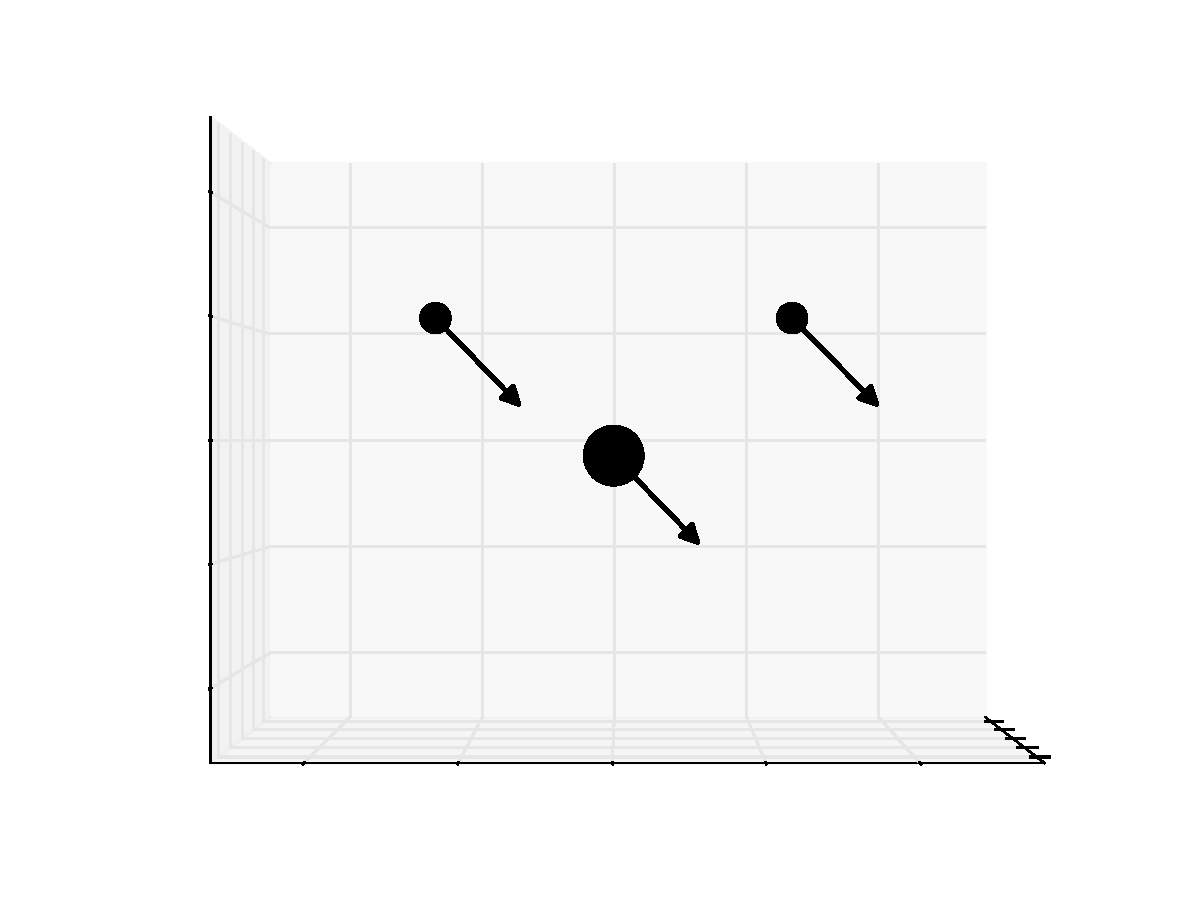
\includegraphics[width=5.5cm,clip=true,trim=3cm 2cm 3cm 2cm]{images/0-0_0.pdf}&
    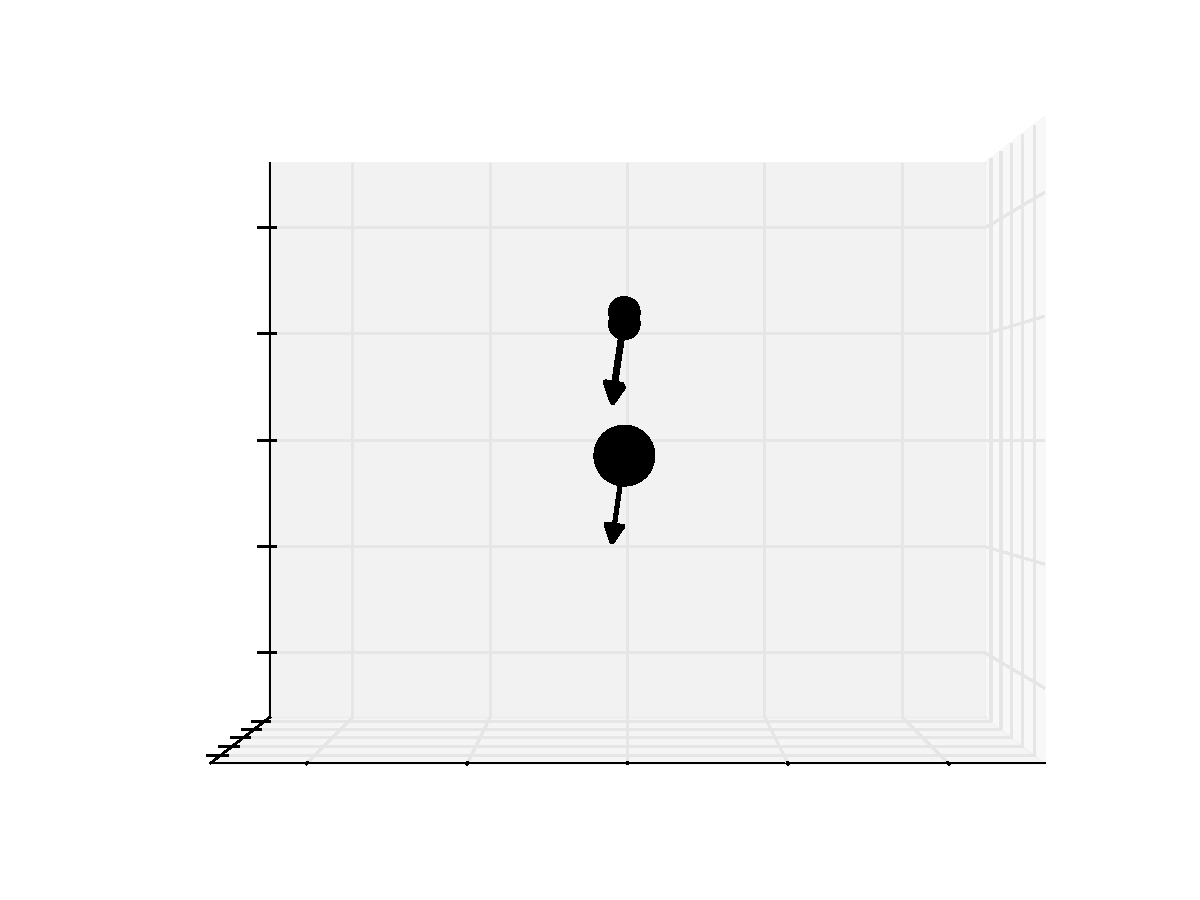
\includegraphics[width=5.5cm,clip=true,trim=3cm 2cm 3cm 2cm]{images/0-90_0.pdf}&
    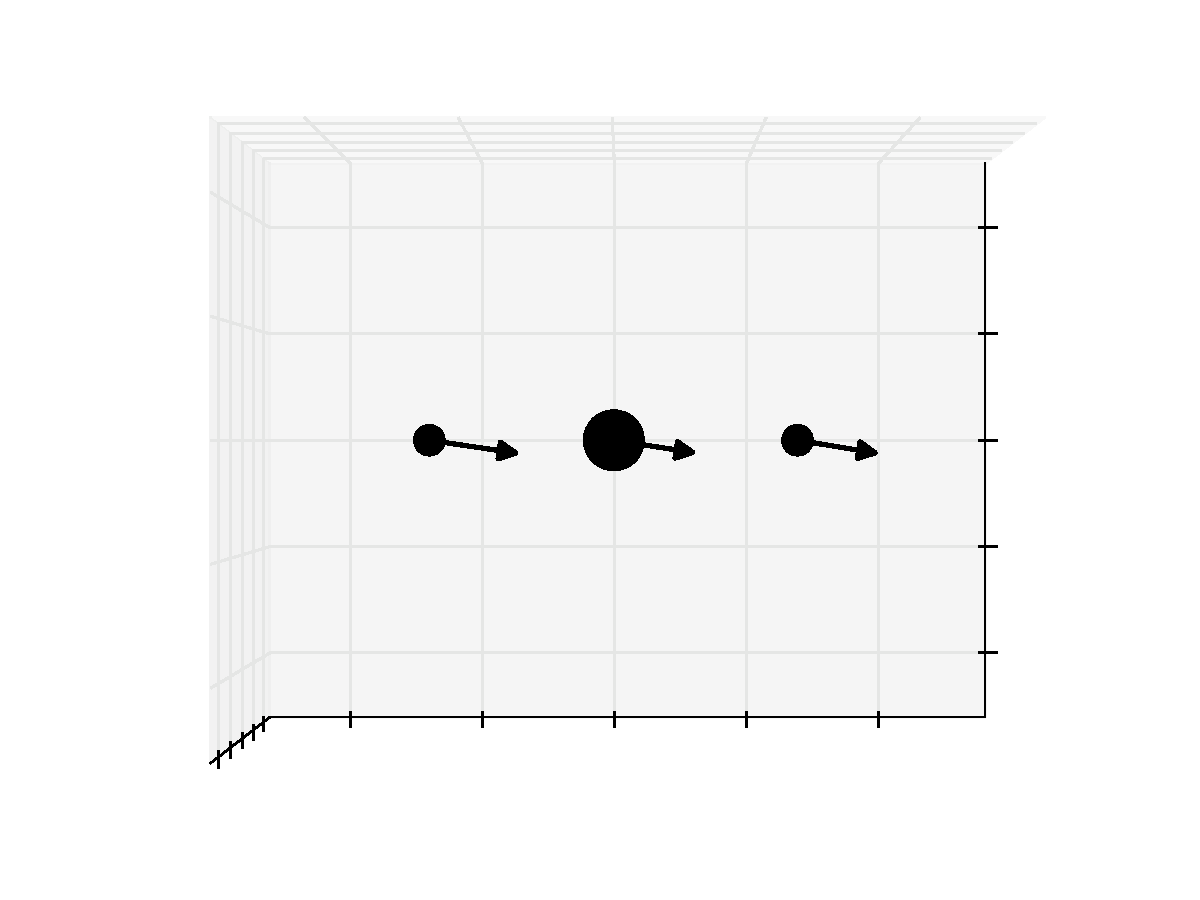
\includegraphics[width=5.5cm,clip=true,trim=3cm 2cm 3cm 2cm]{images/90-0_0.pdf}\\front view&side view&top view\\\hline&&\\
    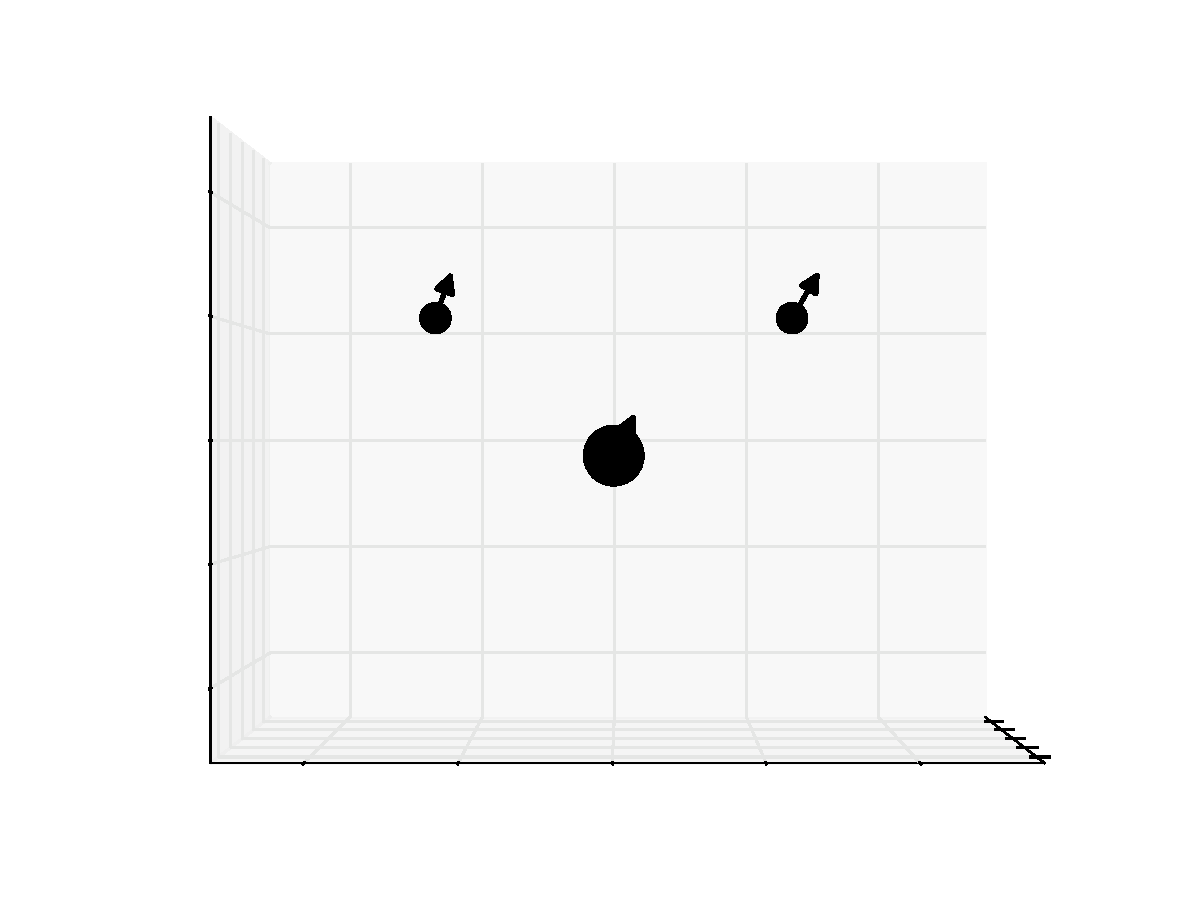
\includegraphics[width=5.5cm,clip=true,trim=3cm 2cm 3cm 2cm]{images/0-0_1.pdf}&
    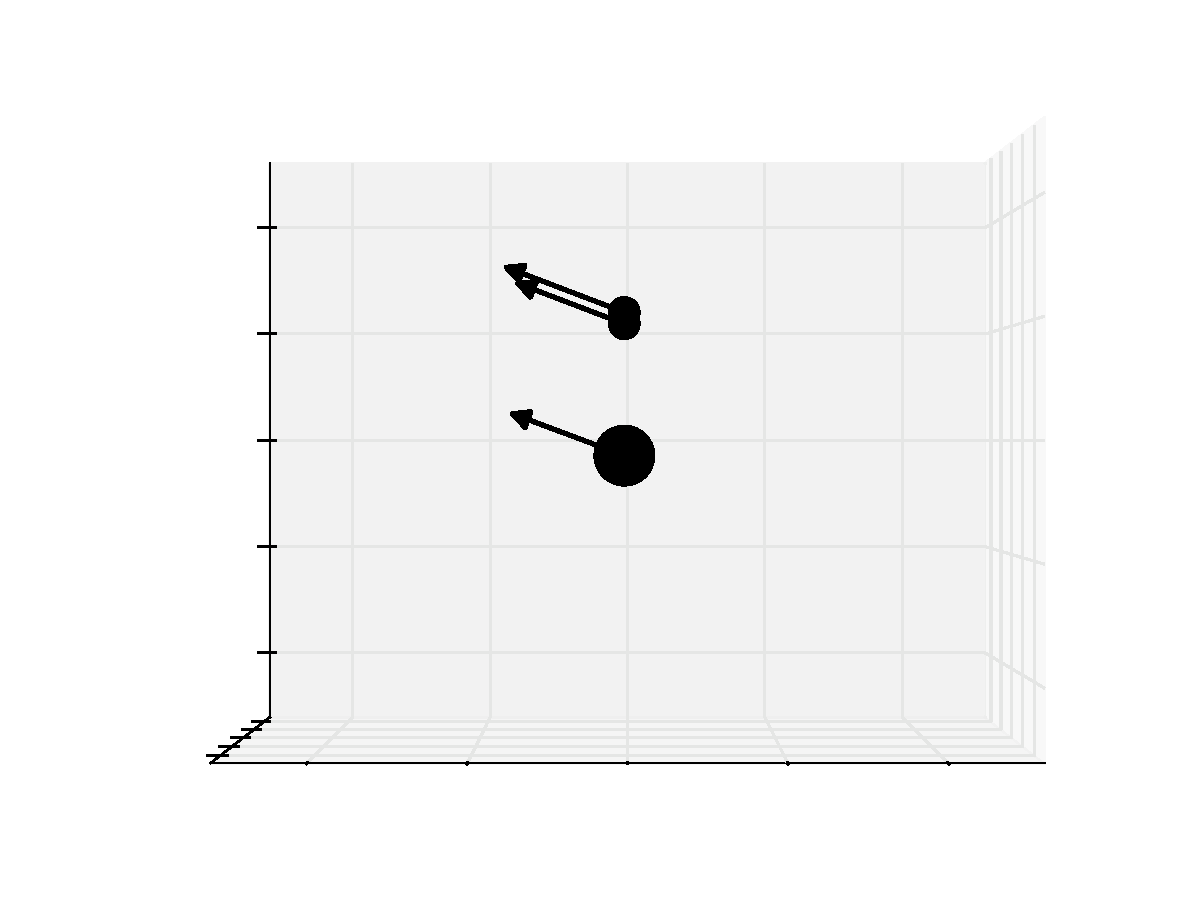
\includegraphics[width=5.5cm,clip=true,trim=3cm 2cm 3cm 2cm]{images/0-90_1.pdf}&
    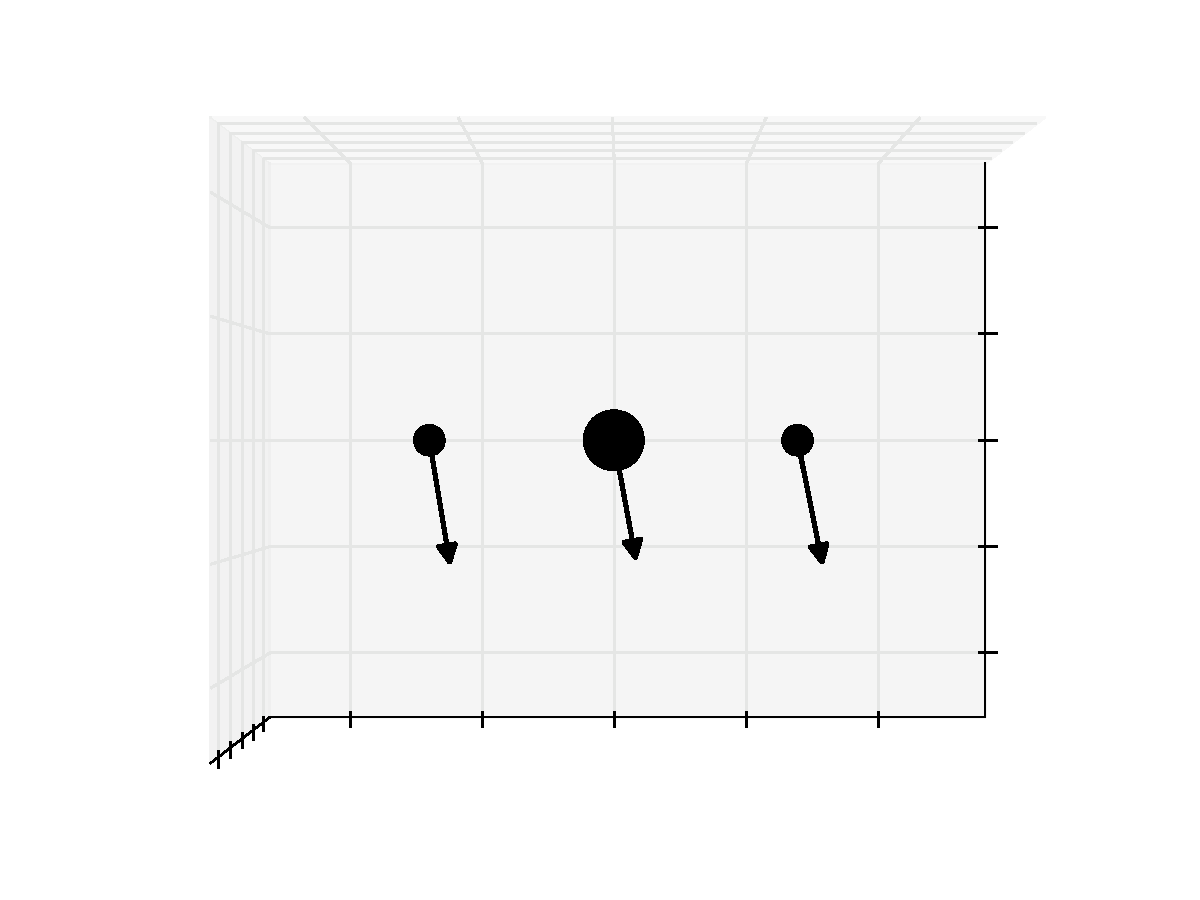
\includegraphics[width=5.5cm,clip=true,trim=3cm 2cm 3cm 2cm]{images/90-0_1.pdf}\\front view&side view&top view\\\hline&&\\
    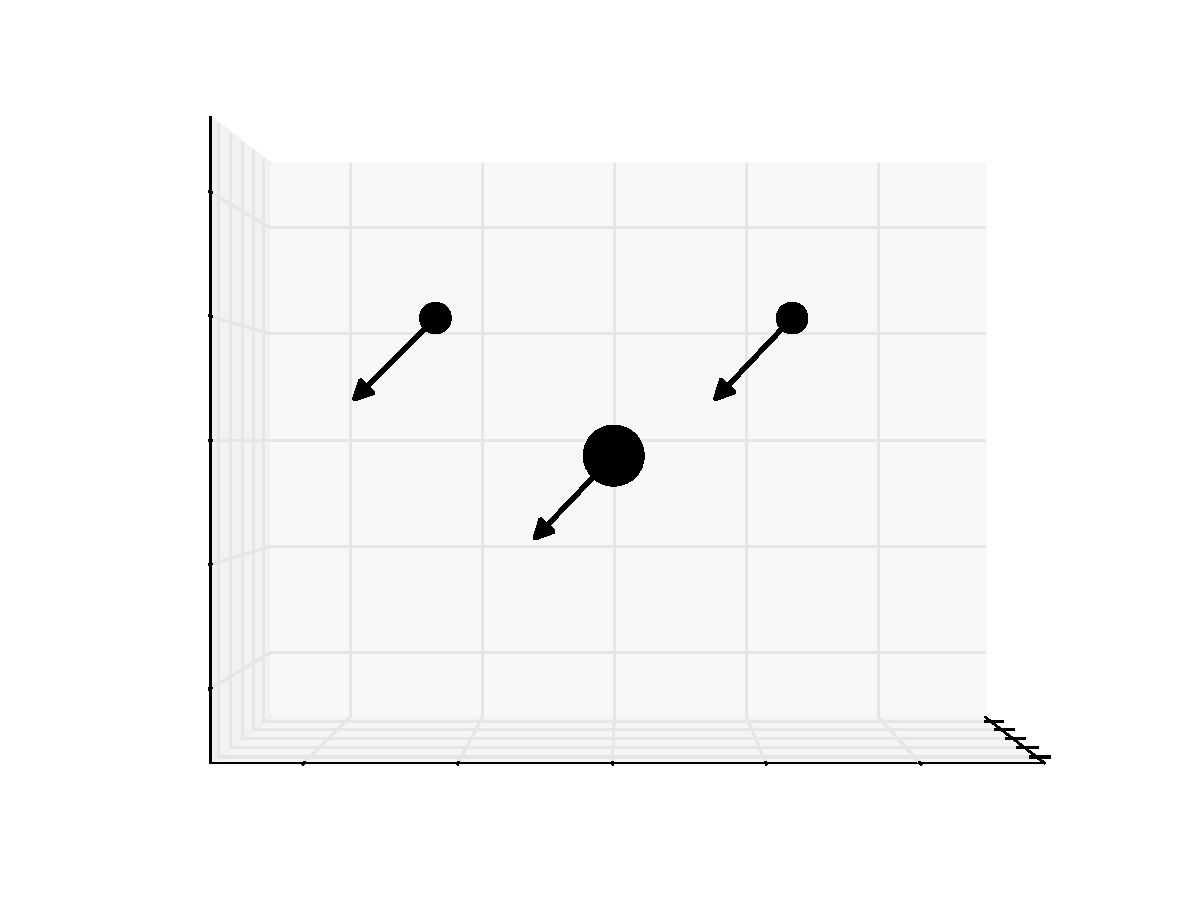
\includegraphics[width=5.5cm,clip=true,trim=3cm 2cm 3cm 2cm]{images/0-0_2.pdf}&
    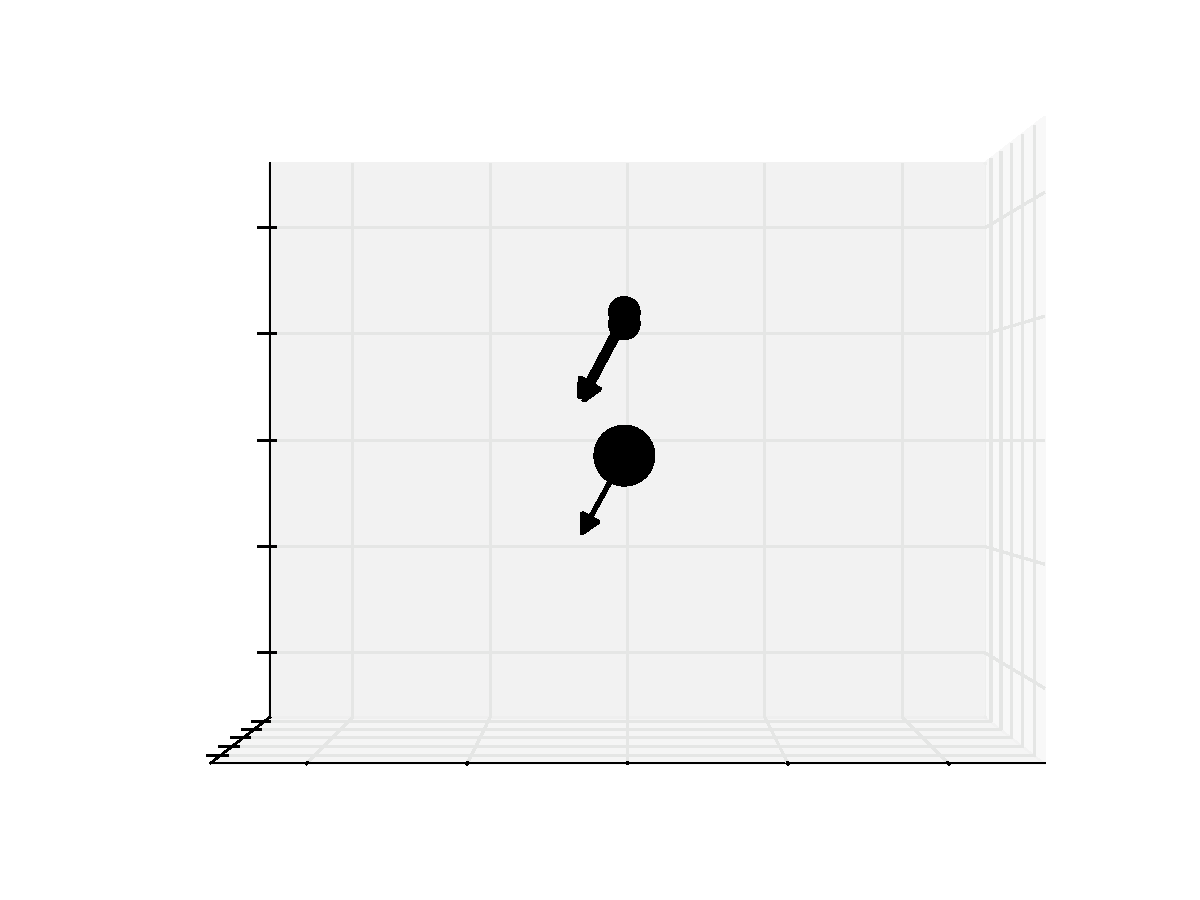
\includegraphics[width=5.5cm,clip=true,trim=3cm 2cm 3cm 2cm]{images/0-90_2.pdf}&
    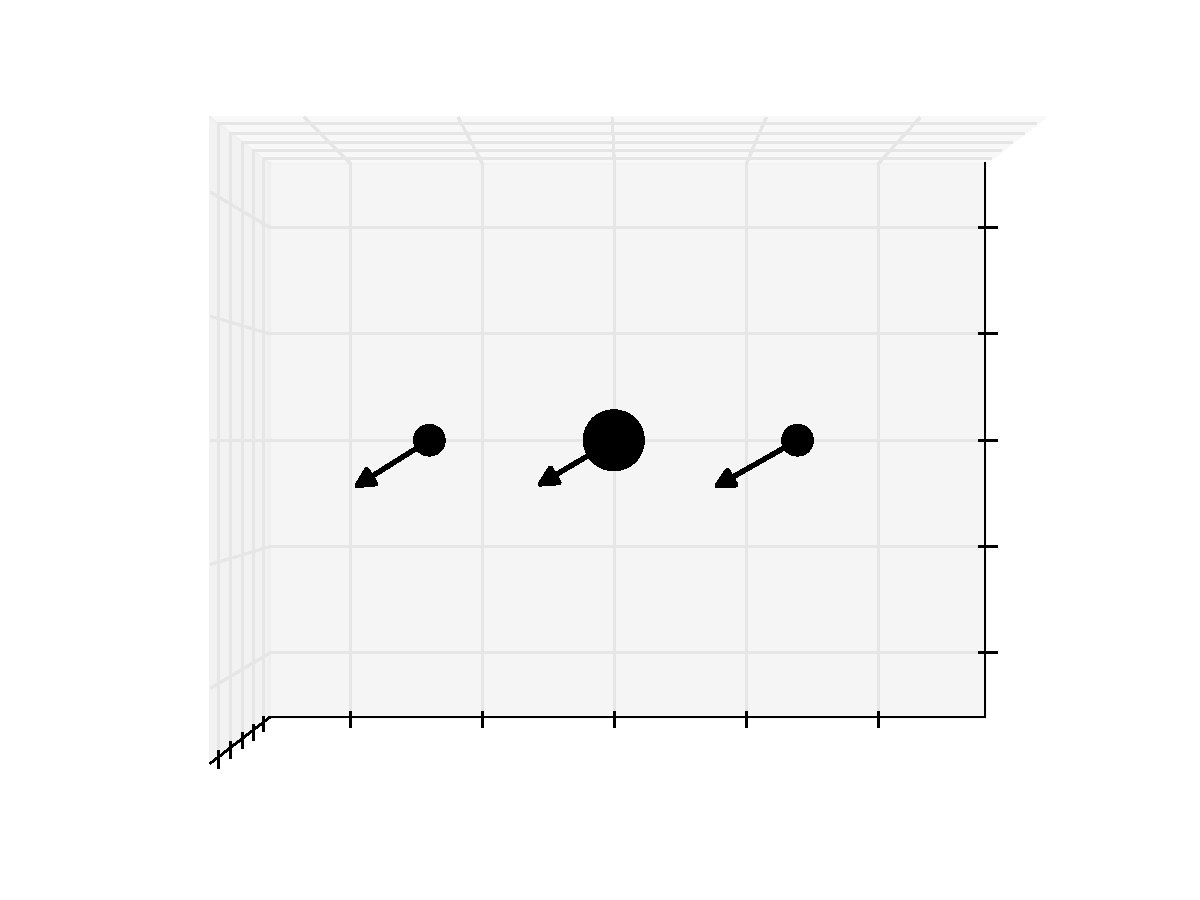
\includegraphics[width=5.5cm,clip=true,trim=3cm 2cm 3cm 2cm]{images/90-0_2.pdf}\\front view&side view&top view\\\hline
    \end{tabular}
\end{figure}
\newpage
\subsubsection{Rotational Modes}
\label{rot}
\begin{figure}[htp]
    \centering
    \begin{tabular}{|ccc|}\hline&&\\
    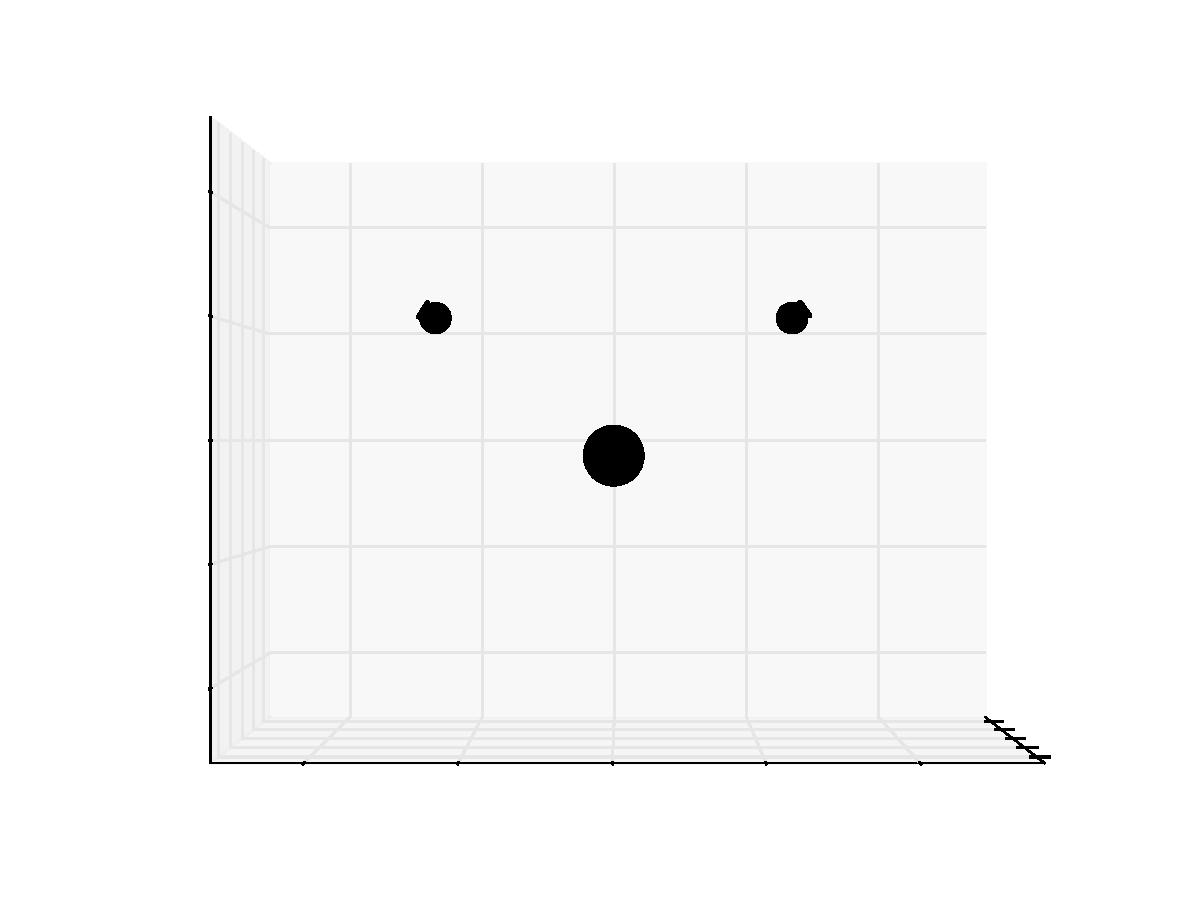
\includegraphics[width=5.5cm,clip=true,trim=3cm 2cm 3cm 2cm]{images/0-0_3.pdf}&
    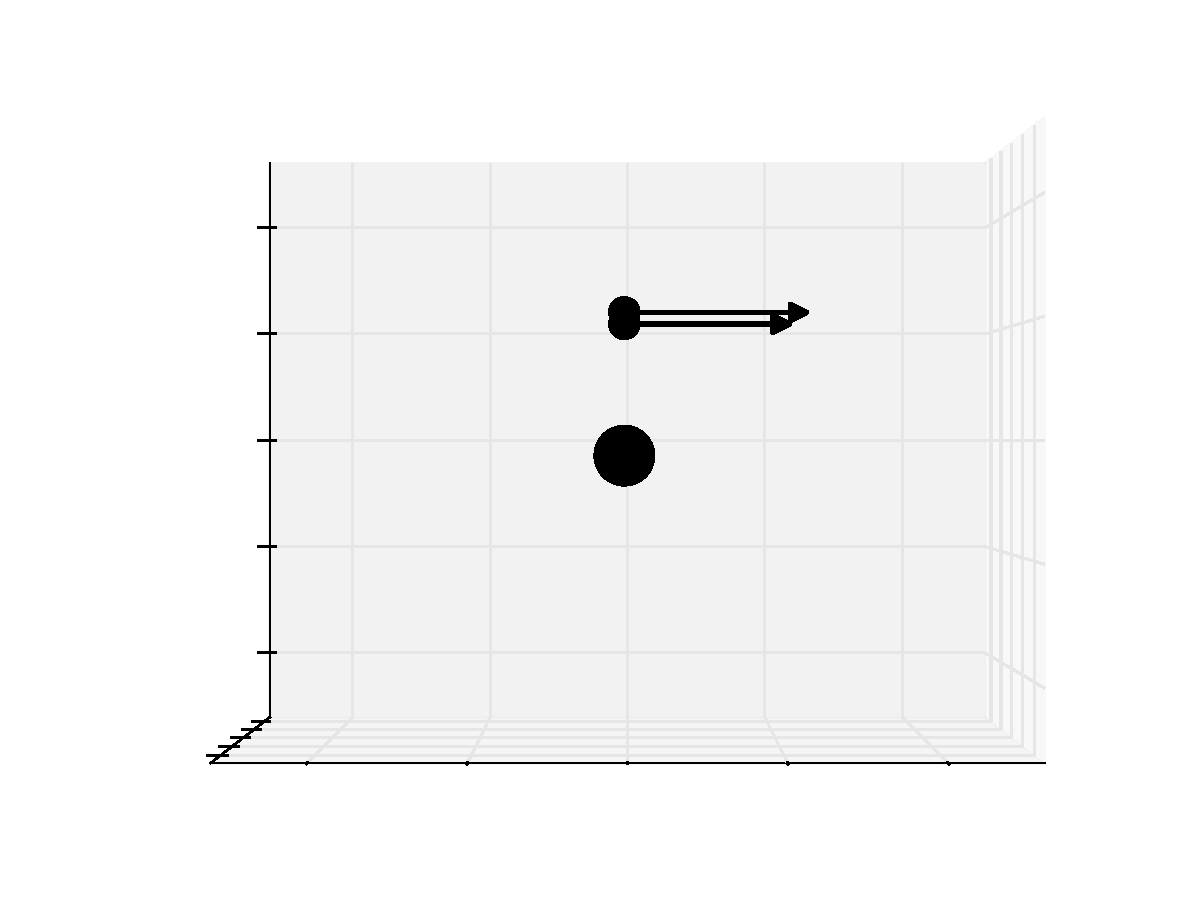
\includegraphics[width=5.5cm,clip=true,trim=3cm 2cm 3cm 2cm]{images/0-90_3.pdf}&
    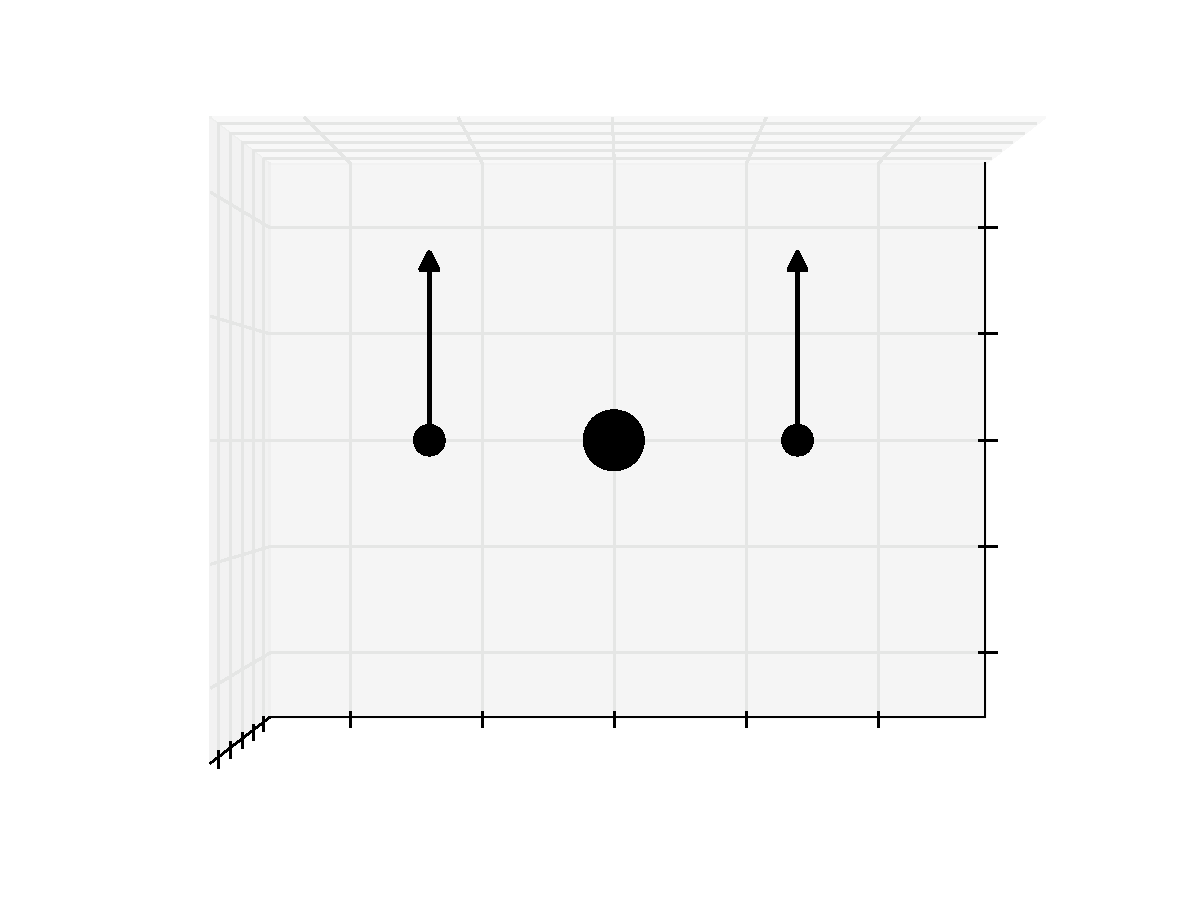
\includegraphics[width=5.5cm,clip=true,trim=3cm 2cm 3cm 2cm]{images/90-0_3.pdf}\\front view&side view&top view\\\hline&&\\
    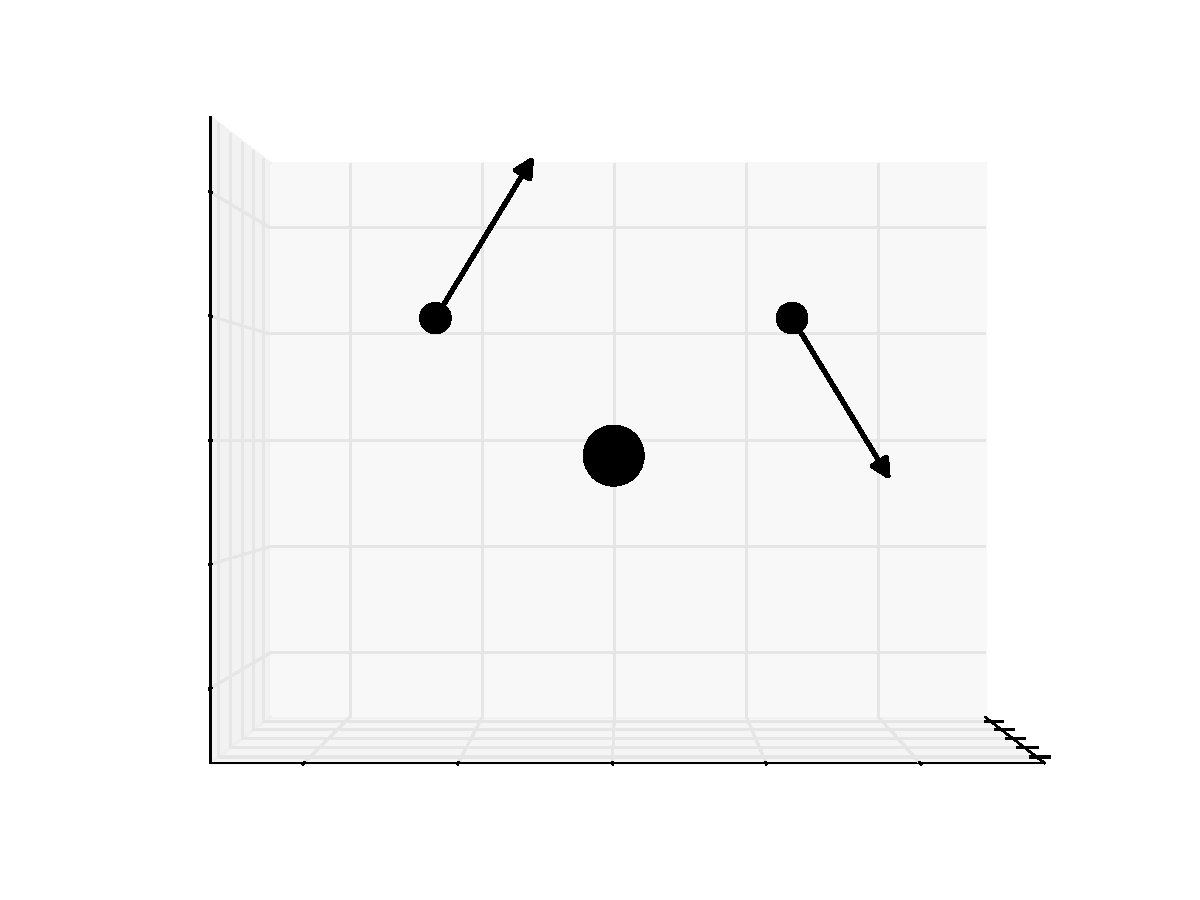
\includegraphics[width=5.5cm,clip=true,trim=3cm 2cm 3cm 2cm]{images/0-0_4.pdf}&
    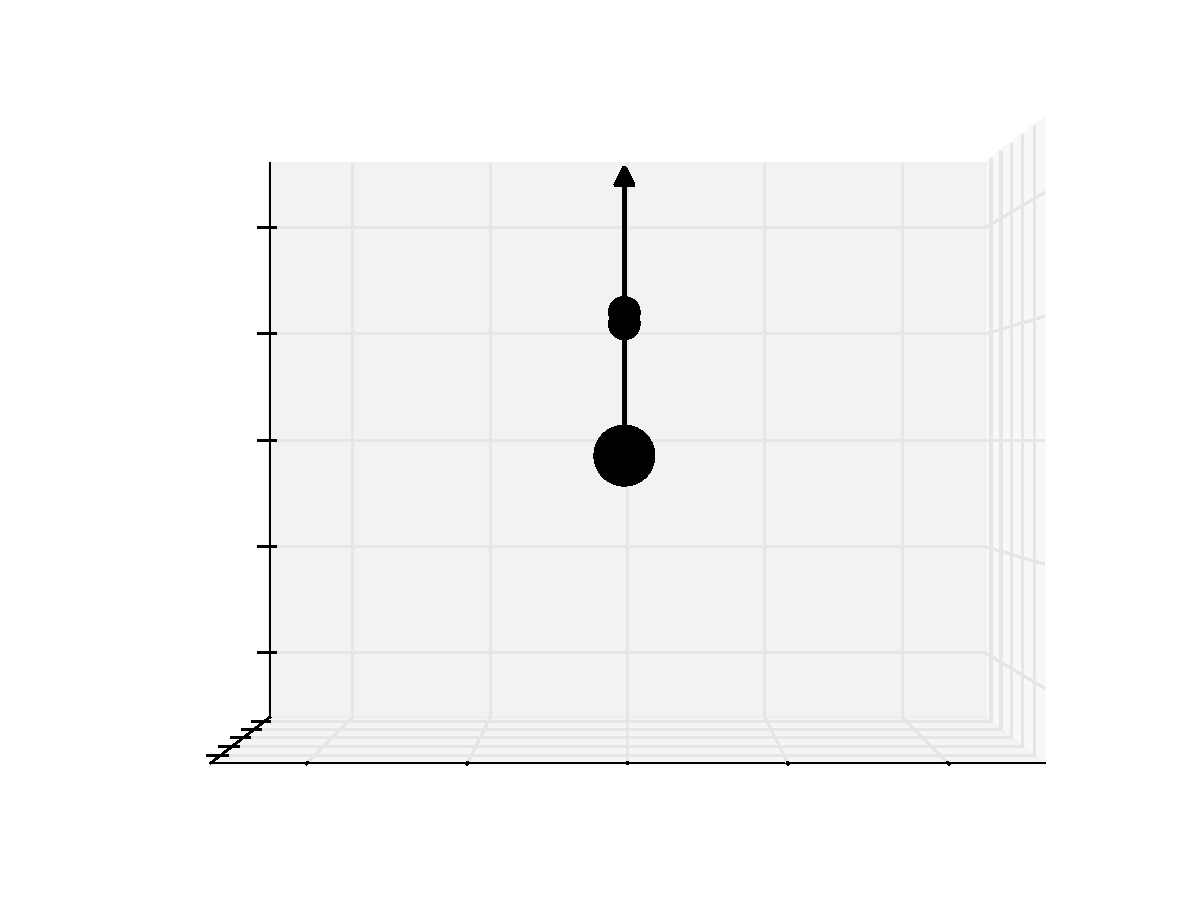
\includegraphics[width=5.5cm,clip=true,trim=3cm 2cm 3cm 2cm]{images/0-90_4.pdf}&
    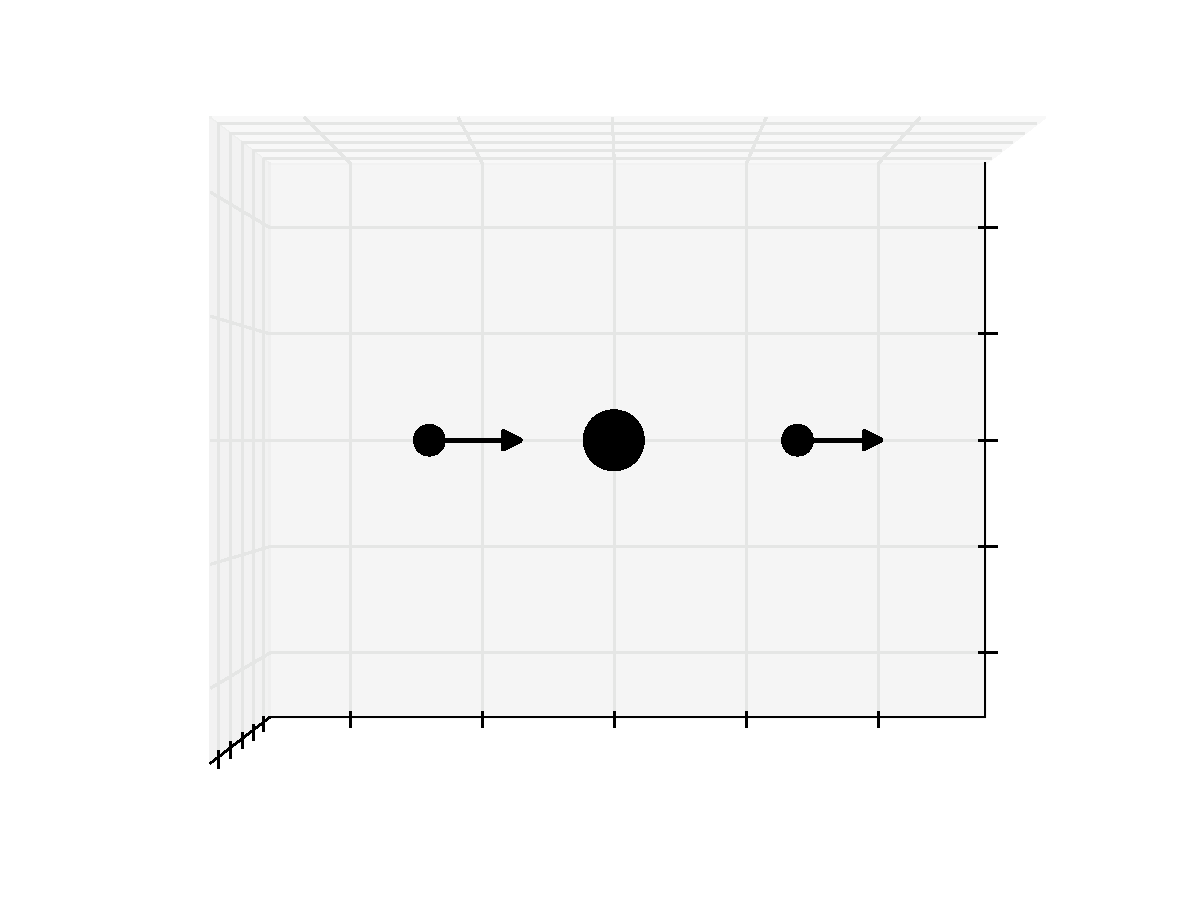
\includegraphics[width=5.5cm,clip=true,trim=3cm 2cm 3cm 2cm]{images/90-0_4.pdf}\\front view&side view&top view\\\hline&&\\
    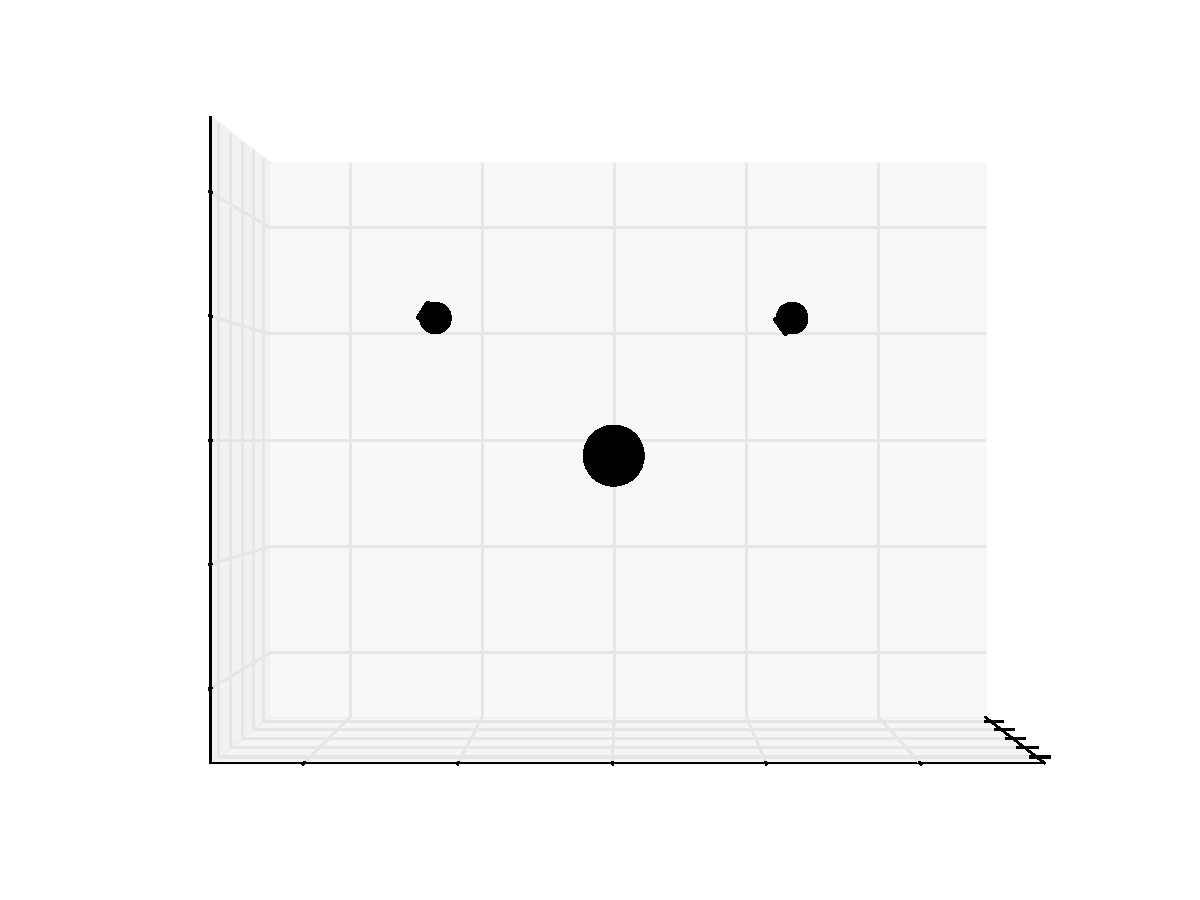
\includegraphics[width=5.5cm,clip=true,trim=3cm 2cm 3cm 2cm]{images/0-0_5.pdf}&
    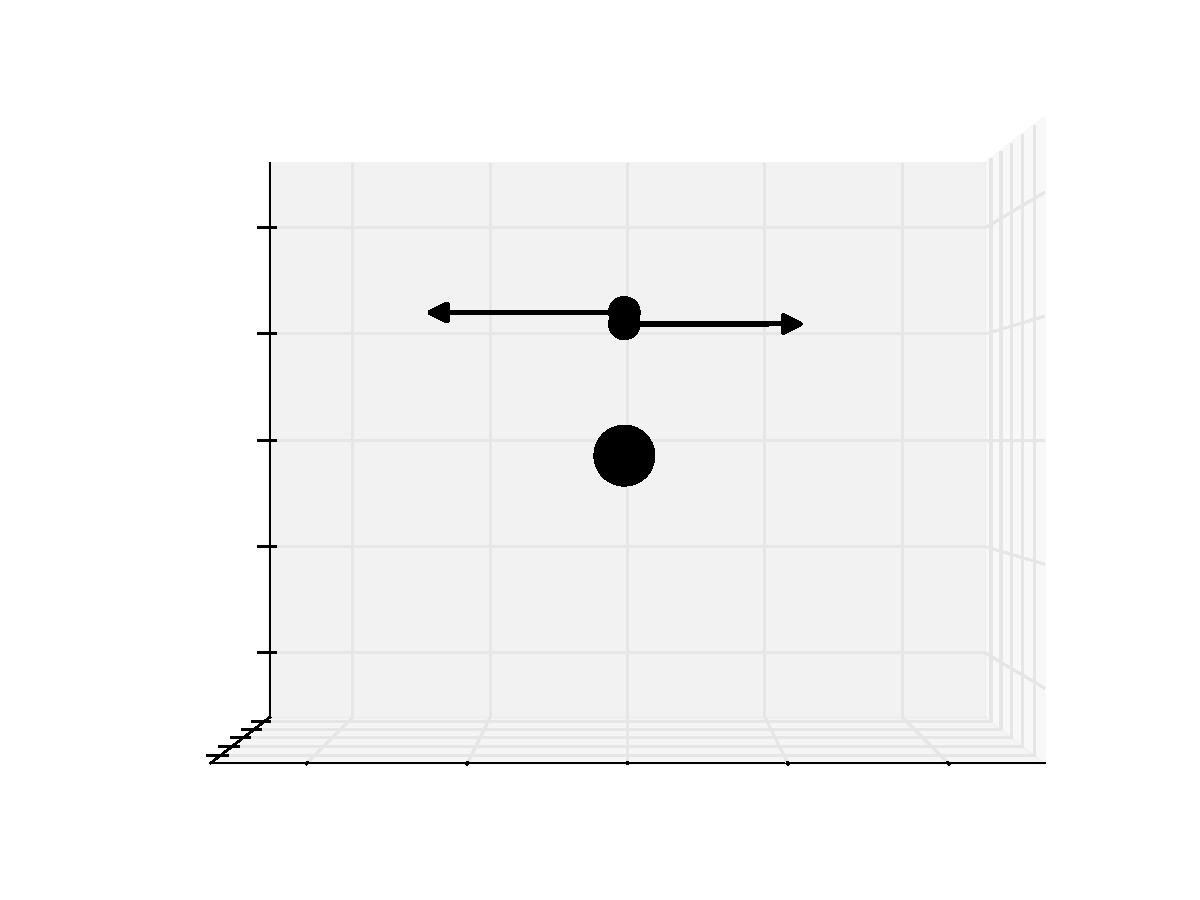
\includegraphics[width=5.5cm,clip=true,trim=3cm 2cm 3cm 2cm]{images/0-90_5.pdf}&
    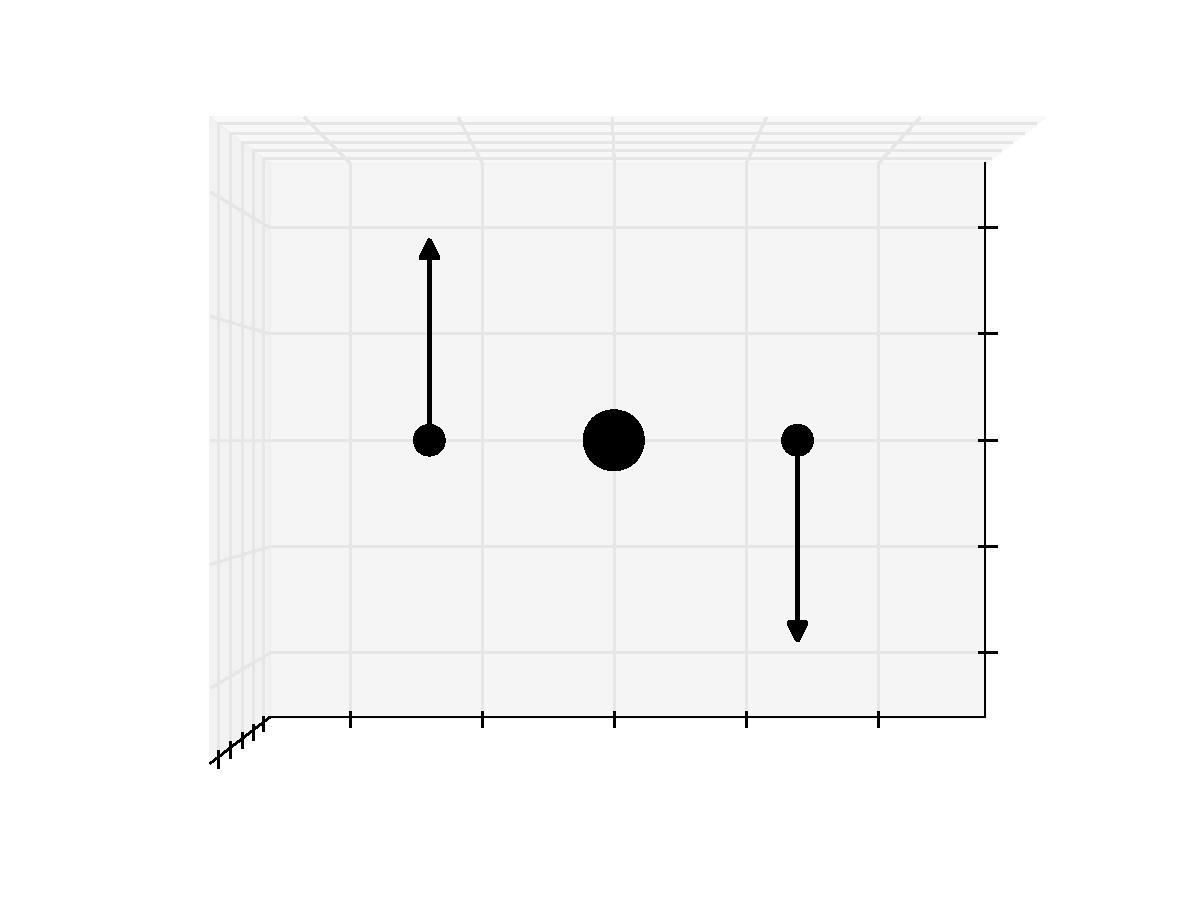
\includegraphics[width=5.5cm,clip=true,trim=3cm 2cm 3cm 2cm]{images/90-0_5.pdf}\\front view&side view&top view\\\hline
    \end{tabular}
\end{figure}
\newpage
\subsubsection{Vibrational Modes}
\label{vib}
\begin{figure}[htp]
    \centering
    \begin{tabular}{|ccc|}\hline&&\\
    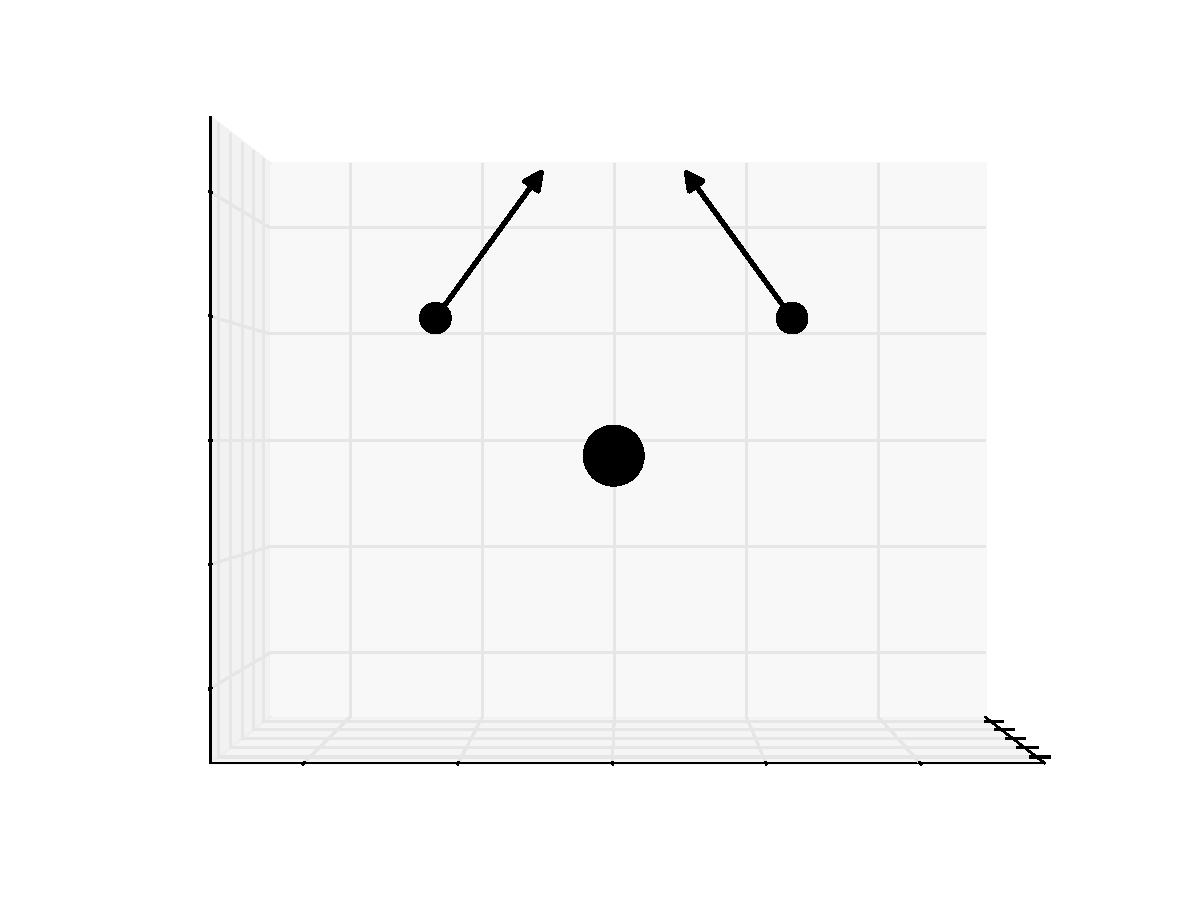
\includegraphics[width=5.5cm,clip=true,trim=3cm 2cm 3cm 2cm]{images/0-0_6.pdf}&
    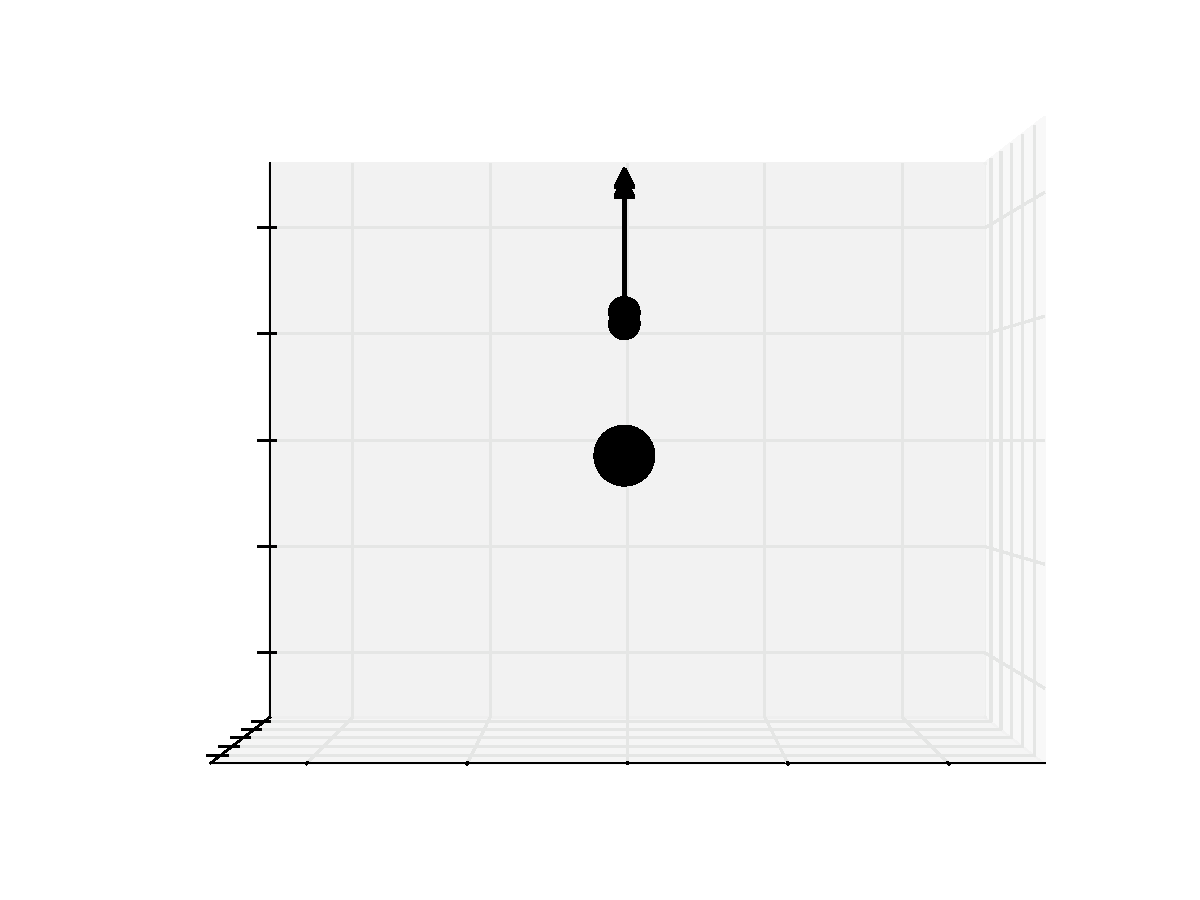
\includegraphics[width=5.5cm,clip=true,trim=3cm 2cm 3cm 2cm]{images/0-90_6.pdf}&
    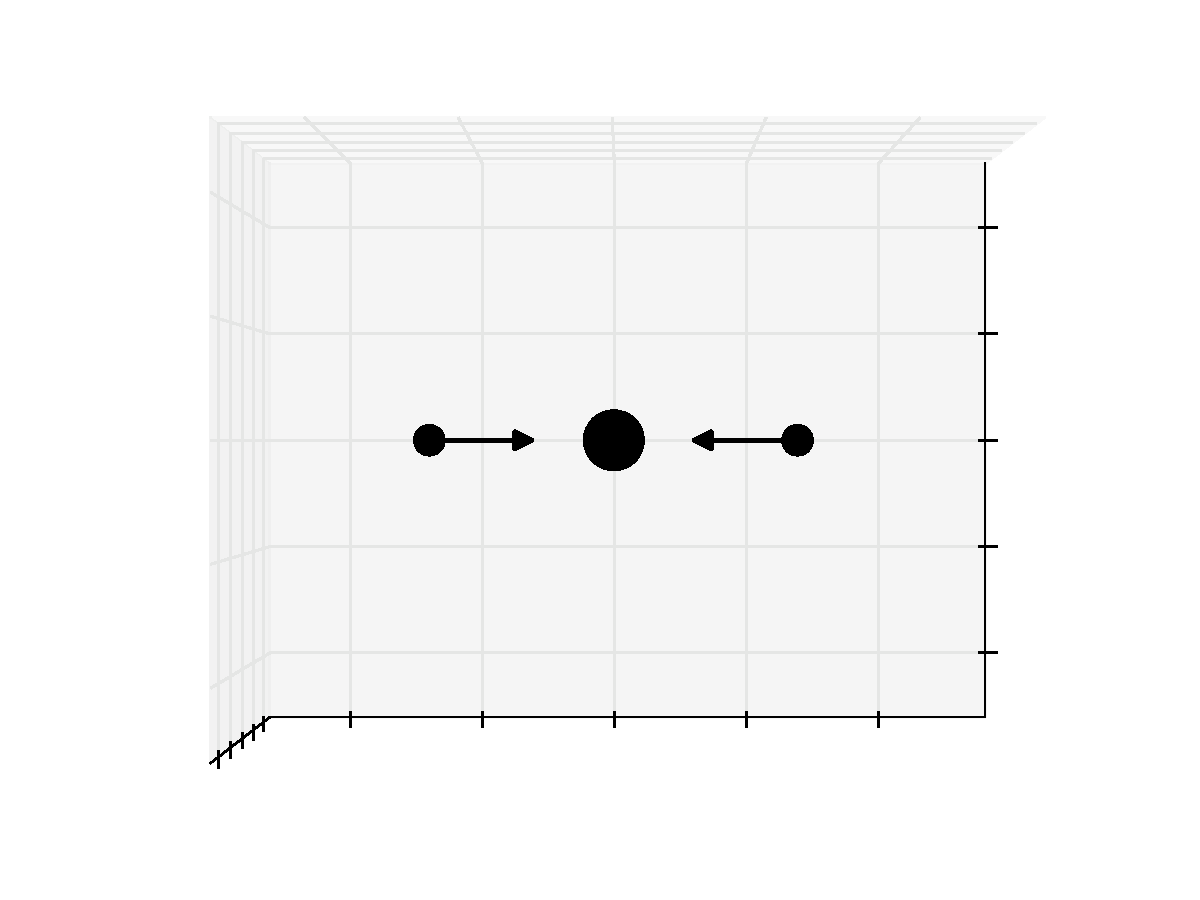
\includegraphics[width=5.5cm,clip=true,trim=3cm 2cm 3cm 2cm]{images/90-0_6.pdf}\\front view&side view&top view\\\hline&&\\
    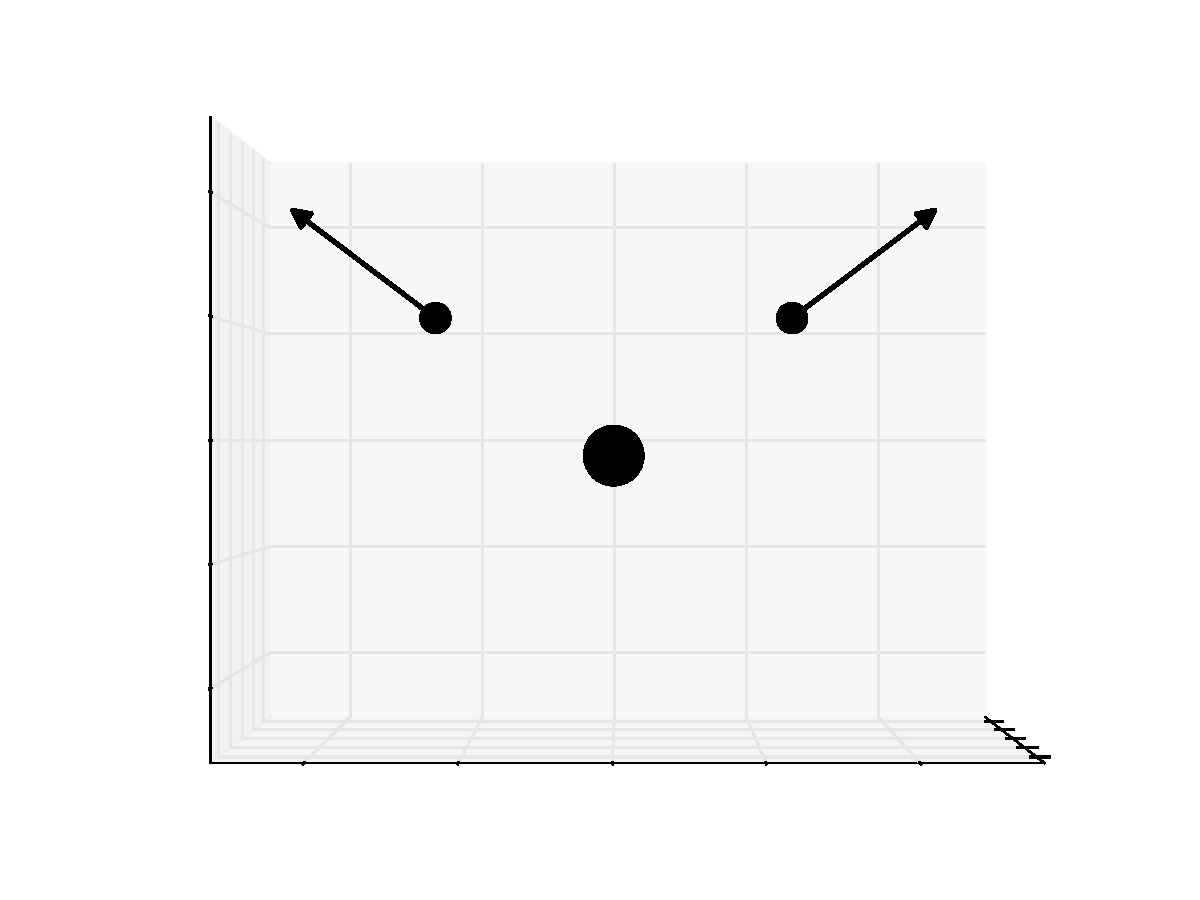
\includegraphics[width=5.5cm,clip=true,trim=3cm 2cm 3cm 2cm]{images/0-0_7.pdf}&
    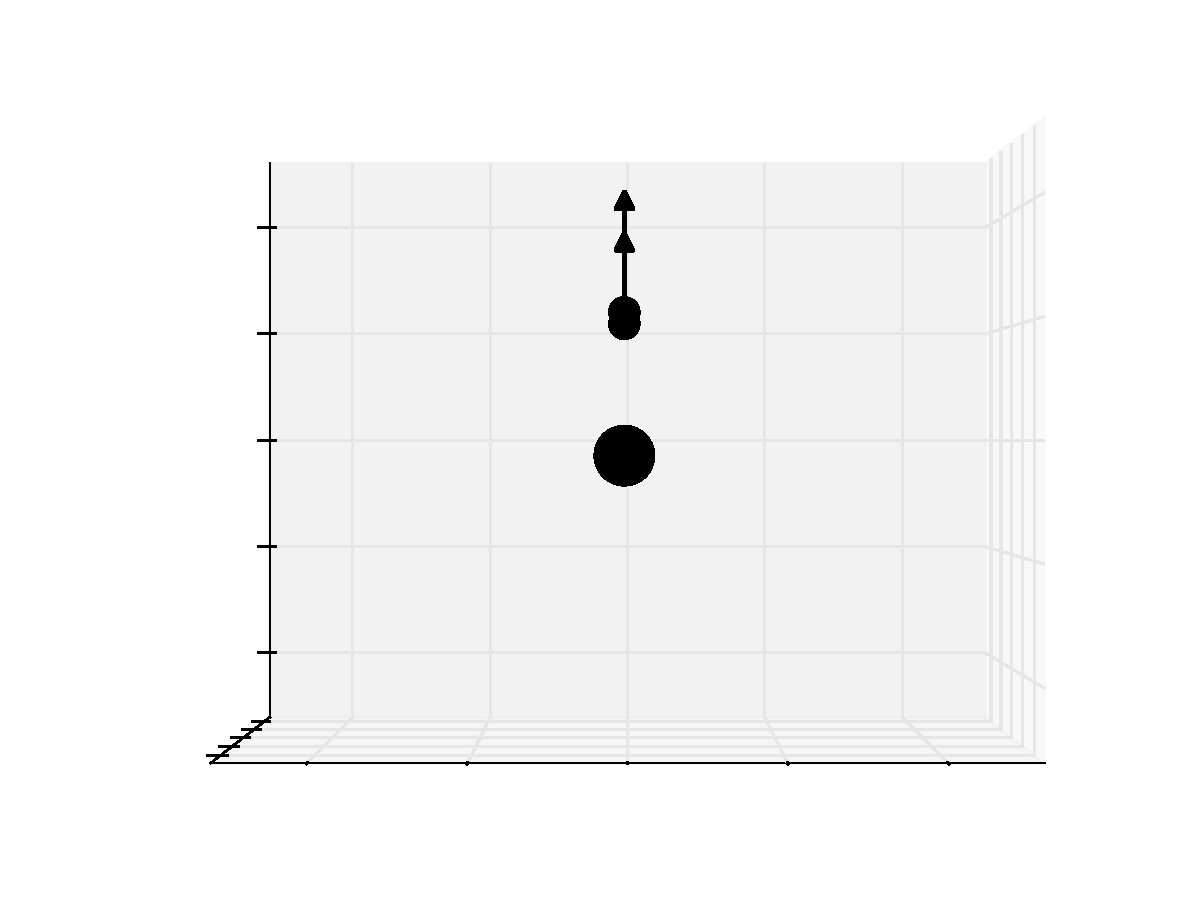
\includegraphics[width=5.5cm,clip=true,trim=3cm 2cm 3cm 2cm]{images/0-90_7.pdf}&
    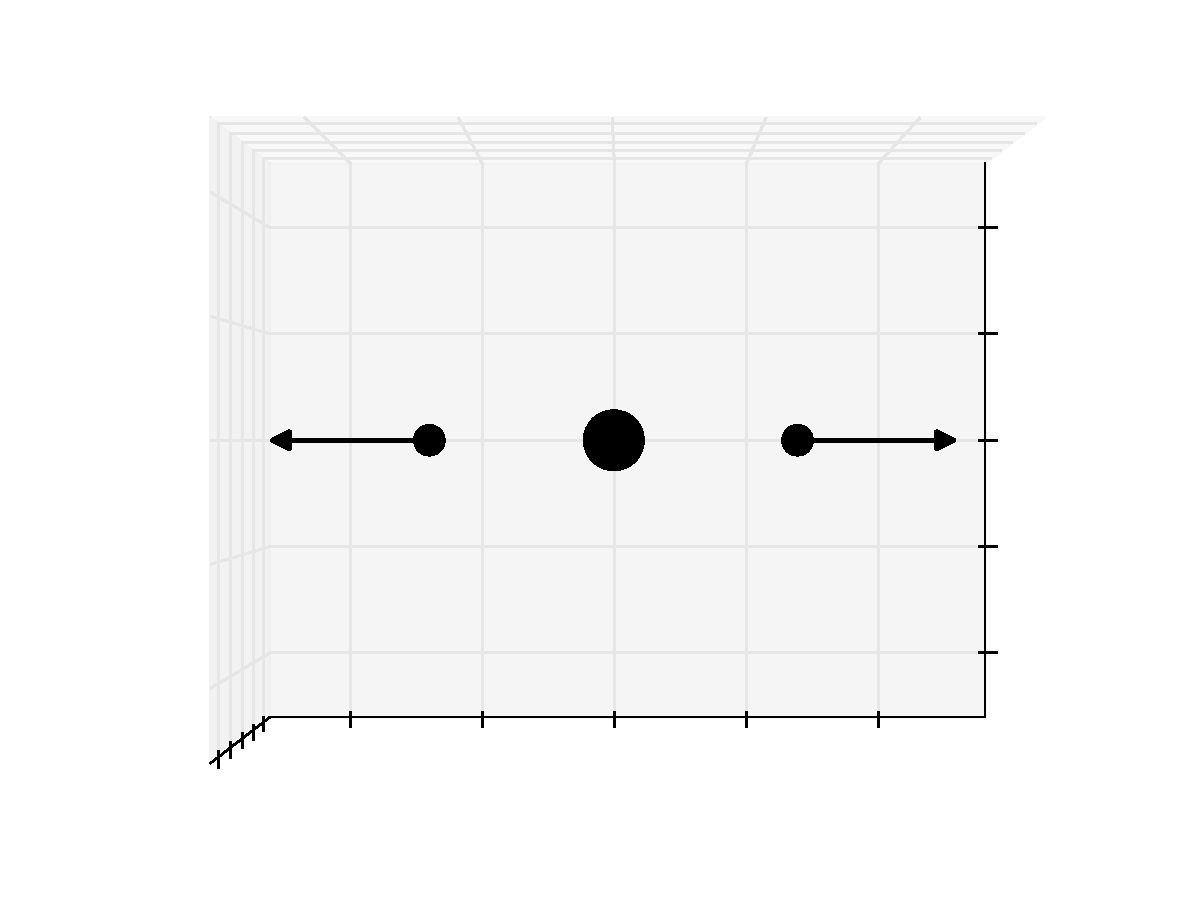
\includegraphics[width=5.5cm,clip=true,trim=3cm 2cm 3cm 2cm]{images/90-0_7.pdf}\\front view&side view&top view\\\hline&&\\
    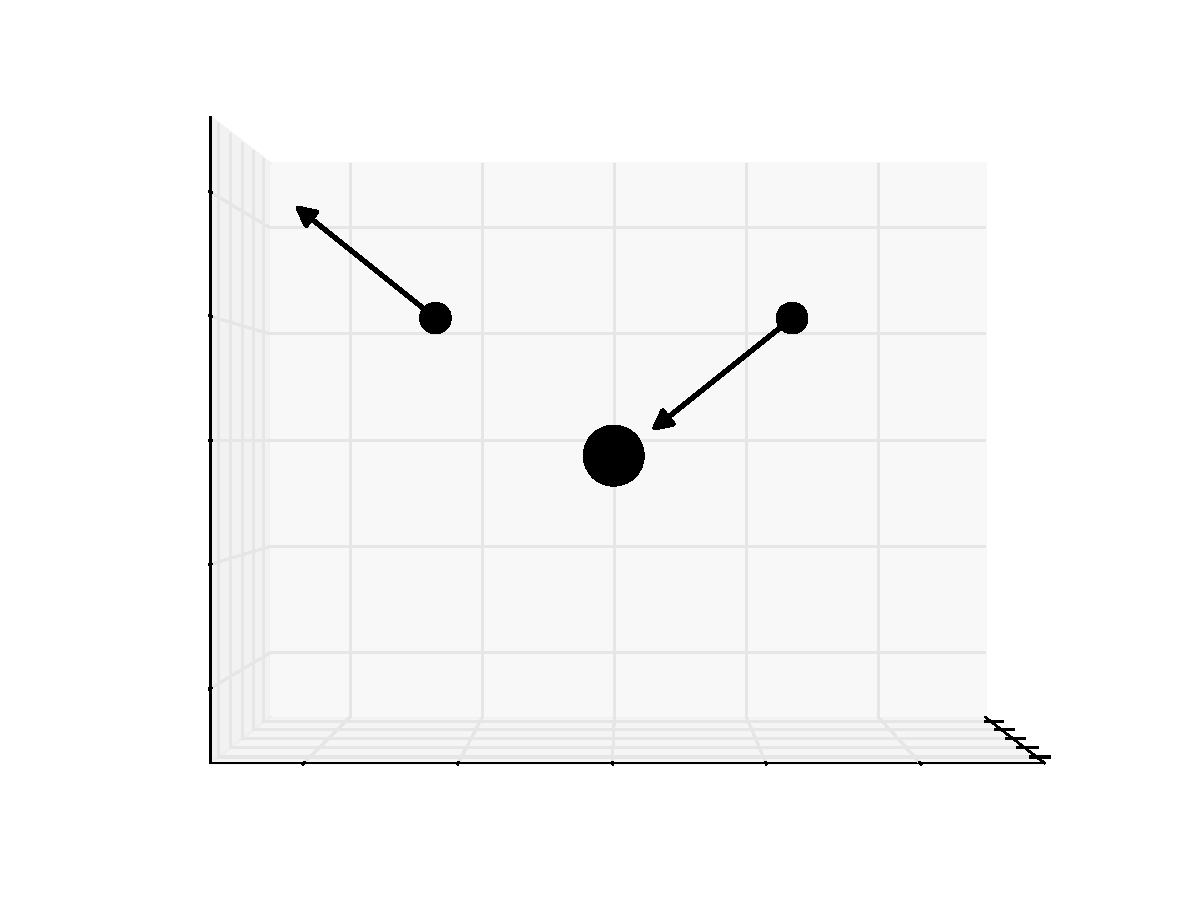
\includegraphics[width=5.5cm,clip=true,trim=3cm 2cm 3cm 2cm]{images/0-0_8.pdf}&
    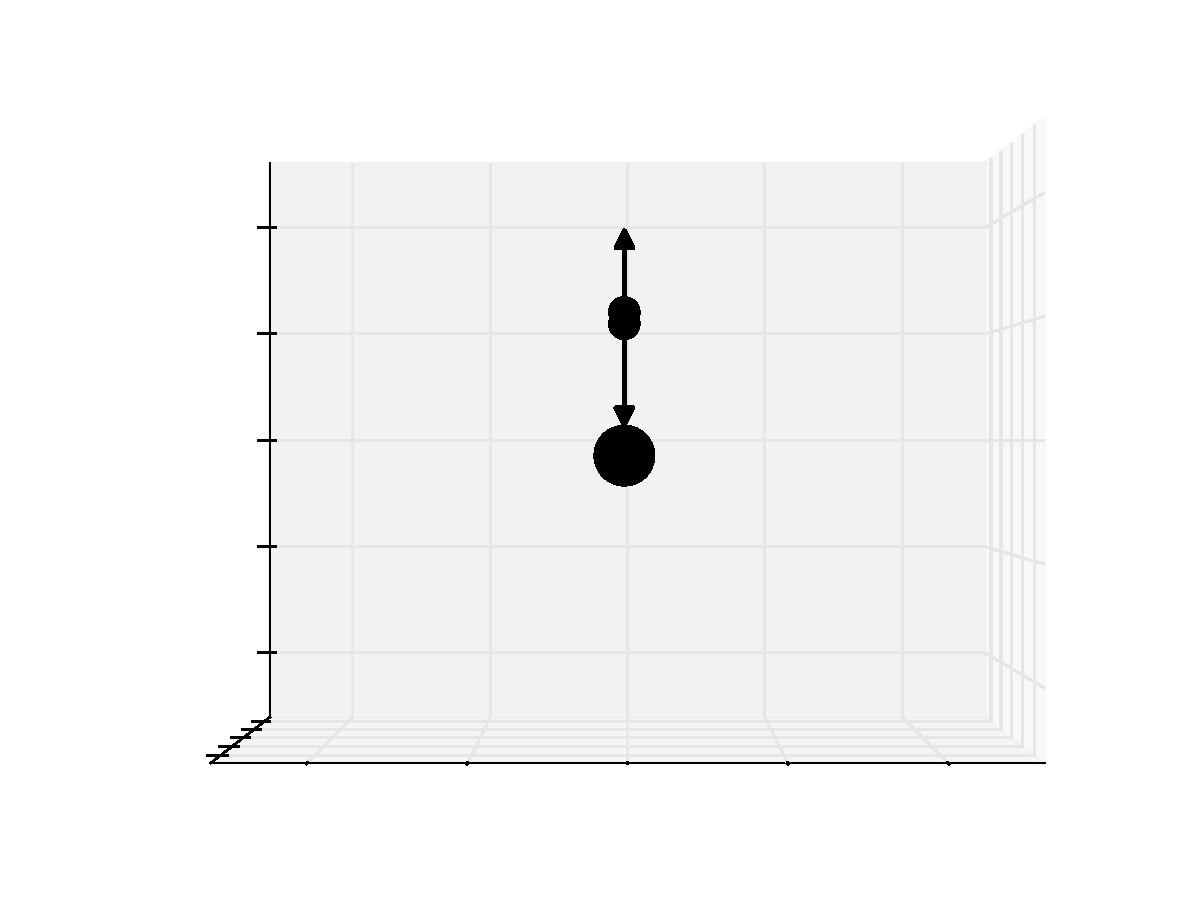
\includegraphics[width=5.5cm,clip=true,trim=3cm 2cm 3cm 2cm]{images/0-90_8.pdf}&
    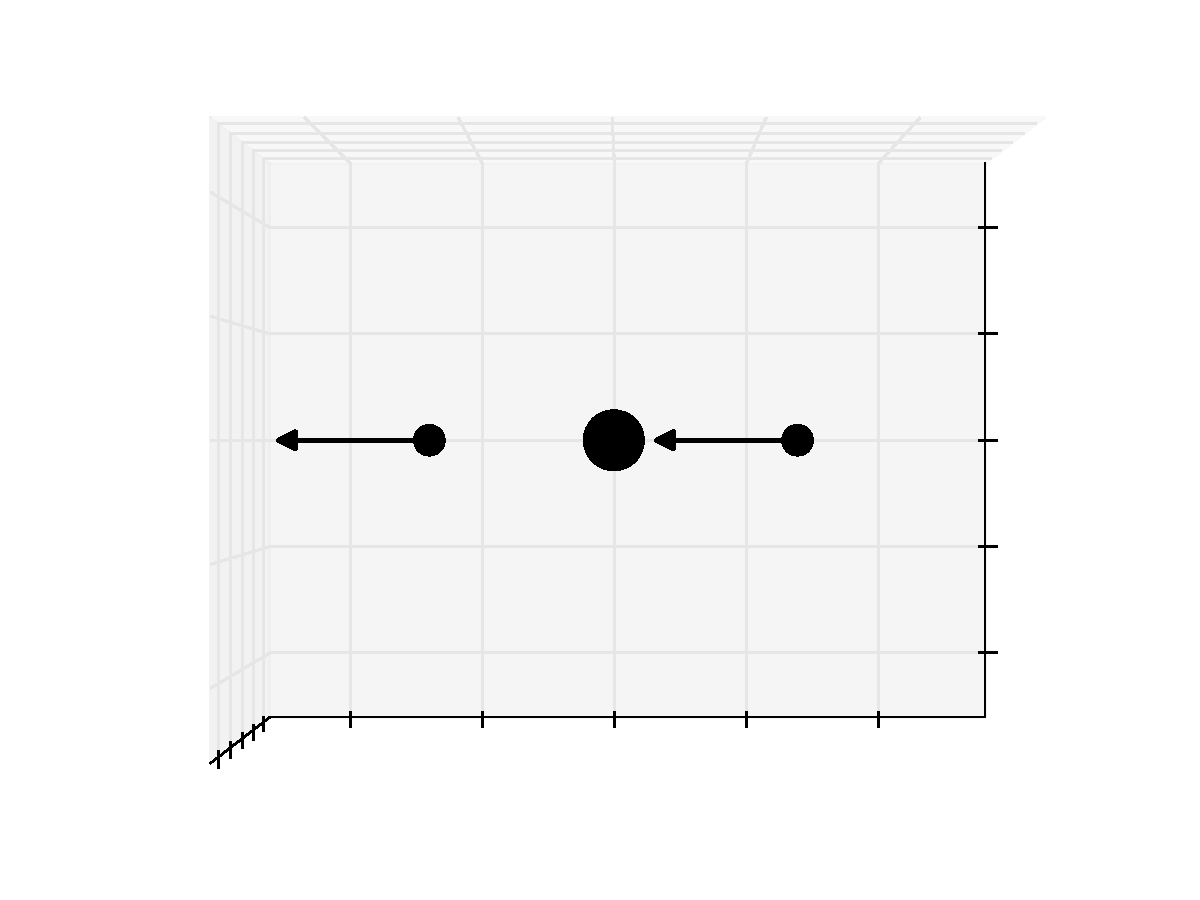
\includegraphics[width=5.5cm,clip=true,trim=3cm 2cm 3cm 2cm]{images/90-0_8.pdf}\\front view&side view&top view\\\hline
    \end{tabular}
\end{figure}

\newpage
\subsection{Appendix: Details of the Coordinate Transformation}
It is worth showing how this coordinate transformation works explicitly. In
particular, we should show how the derivatives transform to arrive at equation
(\ref{vib-se}). Since $\tl{\bo{X}}^T \tl{\bo{H}}_0 \tl{\bo{X}} = (\bo{L}^T
\tl{\bo{X}})^T \bm\La \bo{L}^T \tl{\bo{X}}$, the normal coordinates are given
in terms of mass-weighted Cartesian displacements as
\begin{align*}
    \bo{Q}
=
    \bo{L}^T\tl{\bo{X}}
\end{align*}
or
\begin{align}
%
    Q_A(\tl{X}_1,\ld,\tl{X}_{3N})
=
\sum_{B=1}^{3N}
    L_{BA}
    \tl{X}_B
\end{align}
Then the derivative with respect to $\tl{X}_A$ can be expressed in terms of
derivatives with respect to normal coordinates $\{Q_A\}$ as
\begin{align}
\label{derivative-transform}
%
    \pd{}{}{\tl{X}_A}
=&\
\sum_B
    \pd{}{Q_B}{\tl{X}_A}\pd{}{}{Q_B}
=
\sum_{BC}
    \pd{}{L_{CB}\tl{X}_C}{\tl{X}_A}\pd{}{}{Q_B}
=
\sum_{B}
    L_{AB}\pd{}{}{Q_B}
\end{align}
where we have used the fact that
\begin{align*}
\pd{}{\tl{X}_C}{\tl{X}_A}=\d_{CA}
\end{align*}
($\d_{CA}$ being the Kronecker delta
\footnote{\url{http://en.wikipedia.org/wiki/Kronecker_delta}}). Then we can see
that the kinetic energy operator transforms as follows.
\begin{align*}
\sum_A
    \pd{2}{}{\tl{X}_A}
=
\sum_{ABC}
    \fr{\pt^2}{\pt Q_B\pt Q_C}
    L_{AB}L_{AC}
=
\sum_{BC}
    \fr{\pt^2}{\pt Q_B\pt Q_C}
    (\bo{L}^T\bo{L})_{BC}
\end{align*}
Since $\bo{L}$ is an orthogonal matrix,
$(\bo{L}^T\bo{L})_{BC}=(\bo{1})_{BC}=\d_{BC}$, and so
\begin{align}
%
    \op{T}_\Nu
=
-\fr{1}{2}\sum_A
    \pd{2}{}{\tl{X}_A}
=
-\fr{1}{2}\sum_B
    \pd{2}{}{Q_B} \ \ .
\end{align}
In a similar fashion, we can verify that the transformed Hessian matrix is in
fact simply the Hessian with respect to normal coordinates by comparing
\begin{align*}
%
    \pr{\fr{\pt^2E_e}{\pt\tl{X}_A\pt\tl{X}_B}}_0
=
\sum_{CD}
    \pr{\fr{\pt^2E_e}{\pt Q_C\pt Q_D}}_0
    L_{AC}L_{BD}
\end{align*}
to
\begin{align*}
%
    \pr{\fr{\pt^2E_e}{\pt\tl{X}_A\pt\tl{X}_B}}_0
=
    (\tl{\bo{H}}_0)_{AB}
=
    (\bo{L}\bm\La\bo{L}^T)_{AB}
=
    \sum_{CD}
    (\la_C\d_{CD})L_{AC}L_{BD}
\end{align*}
which shows that
\begin{align}
%
    \pr{\fr{\pt^2E_e}{\pt Q_C\pt Q_D}}_0
=
    \la_C\d_{CD}
\end{align}
That is, we have identified the diagonal elements $\{\la_A\}$ of $\bm\La$ as corresponding to
\begin{align}
    \la_A \equiv \pr{\pd{2}{E_e}{Q_A}}_0
\end{align}
and shown that mixed derivatives are zero
\begin{align}
    \pr{\fr{\pt^2E_e}{\pt Q_A\pt Q_B}}_0
=
    0
\sp
    \text{ if } A\neq B \ .
\end{align}

\end{document}
